%\documentclass[preprint,5p]{elsarticle}
\documentclass[preprint,3p]{elsarticle}

%\usepackage{ecrc}
%% The ecrc package defines commands needed for running heads and logos.
%% For running heads, you can set the journal name, the volume, the starting page and the authors

%\volume{00}
%\firstpage{1}
%% Give the name of the journal
\journal{Nuclear Instruments and Methods}



%% The choice of journal logo is determined by the \jid and \jnltitlelogo commands.
%% A user-supplied logo with the name <\jid>logo.pdf will be inserted if present.
%% e.g. if \jid{yspmi} the system will look for a file yspmilogo.pdf
%% Otherwise the content of \jnltitlelogo will be set between horizontal lines as a default logo

%% Give the abbreviation of the Journal.
%\jid{procs}

%% Give a short journal name for the dummy logo (if needed)
%\jnltitlelogo{Procedia Computer Science}

%% Hereafter the template follows `elsarticle'.
%% For more details see the existing template files elsarticle-template-harv.tex and elsarticle-template-num.tex.

%% Elsevier CRC generally uses a numbered reference style
%% For this, the conventions of elsarticle-template-num.tex should be followed (included below)
%% If using BibTeX, use the style file elsarticle-num.bst

%% End of ecrc-specific commands
%%%%%%%%%%%%%%%%%%%%%%%%%%%%%%%%%%%%%%%%%%%%%%%%%%%%%%%%%%%%%%%%%%%%%%%%%%
\usepackage{geometry}
\usepackage[parfill]{parskip}   
\usepackage{graphicx}
\usepackage{amsmath}
\usepackage[]{color}
%\usepackage[separate-uncertainty=true, range-phrase = --,
%range-units=single, per-mode=symbol]{siunitx}
\usepackage{booktabs}

\setlength{\textwidth}{7.0in}
\setlength{\textheight}{9in} 
\setlength{\oddsidemargin}{-.25in}
\setlength{\evensidemargin}{-0.25in} 
\setlength{\topmargin}{-0.6in}
\setlength{\parskip}{3ex plus 0.5ex minus 0.2ex}

%% The amssymb package provides various useful mathematical symbols
\usepackage{amssymb}
%% The amsthm package provides extended theorem environments
\usepackage{amsthm}

%% The lineno packages adds line numbers. Start line numbering with
%% \begin{linenumbers}, end it with \end{linenumbers}. Or switch it on
%% for the whole article with \linenumbers after \end{frontmatter}.
\usepackage{lineno}

%% natbib.sty is loaded by default. However, natbib options can be
%% provided with \biboptions{...} command. Following options are
%% valid:

%%   round  -  round parentheses are used (default)
%%   square -  square brackets are used   [option]
%%   curly  -  curly braces are used      {option}
%%   angle  -  angle brackets are used    <option>
%%   semicolon  -  multiple citations separated by semi-colon
%%   colon  - same as semicolon, an earlier confusion
%%   comma  -  separated by comma
%%   numbers-  selects numerical citations
%%   super  -  numerical citations as superscripts
%%   sort   -  sorts multiple citations according to order in ref. list
%%   sort&compress   -  like sort, but also compresses numerical citations
%%   compress - compresses without sorting
%%
\biboptions{comma,round,sort&compress,numbers}


% if you have landscape tables
\usepackage[figuresright]{rotating}

% put your own definitions here:
%   \newcommand{\cZ}{\cal{Z}}
%   \newtheorem{def}{Definition}[section]
%   ...

% to add subfigures
\usepackage{caption}
\usepackage{subcaption}

% add words to TeX's hyphenation exception list
\hyphenation{author another created financial paper re-commend-ed Post-Script}

% declarations for front matter

\begin{document}

\graphicspath{{figs/}}

\input{./Title.tex}
%%
%% Start line numbering here if you want
%%
\linenumbers

%% main text
\input{./Intro.tex}

\section{Detailed study of Equipments}

%\begin{figure}
%  \centering
%  \includegraphics[width=4in]{gecko}
%  \caption[Close up of \species{Hemidactylus}]
%  {Close up of \species{Hemidactylus}, which is part the genus of the gecko family. It is the second most 
%    speciose genus in the family.}
%\end{figure}

%\newtheorem{name}{Printed output}



\subsection{Tank}



large grey plastic vessel

Should we line the inner surface? Stan has been investigating various
non-reflective surfaces

needs investigation into water compatibility and possible emanation





\subsection{Mechanical Gantry System}


As noted before in the introduction, the PTF measurements are made by moving a pair of optical heads to
different positions to illuminate the 20\" PMT.  This motion is accomplished by having the optical heads be on
a pair of moveable gantries.  The gantries provide movement in five different axes: X, Y, Z, rotation and tilt.
The X, Y and Z motion is on three separate linear stages driven by stepper motors,
with the dimensions of the stages being XXXYYY, XXXYYY
and XXXYYY.  The tilt motion is provided by a rotary stage; the tilt motion of the optical head is
provided by a XXXYYY driven by a stepper motor.
This is all shown diagramatically in Figure XXXYYY; these elements are all duplicated for
the two gantries.  The gantry motors are controlled by a Galil 8143 motor controller; the controller is configured
over an ethernet link.  The configuration is handled in a MIDAS program and webpage, described in Section
\ref{Sec:DAQ_Controls}.

Limit switches provide some degree of protection against collisions.  But the two gantries can
be moved into the same space; so additional higher-level collision avoidance has been
programmed into the software control programs.



Various tests have been performed to understand the reproducibility of the gantry motion.  This tests have shown
XXXYYY






\subsection{Optical System/Head}

Shimpei

collimate/polarize the incoming light

watertight

how to manipulate?

new sources?



\subsection{Optical Fibre}
ideal wavelength range is 350--650~nm

consider bending radius

throughput

tested three samples

selected FT200UMT

good transmission across the wavelengths tested~(378--777~nm)

seemed almost unaffected by curvature

fibre must reach several metres from laser through manipulator to the
optical head

how to mount, etc. to prevent tangles, excessive bending, etc.


\subsection{Magnetic Field Compensation}

assess magnetic shielding, magnetic compensation

GIRON magnetic shielding (http://www.lessemf.com/)

GIRON frame

Helmholtz coils, could include the dimensions, wire details,
measured resistance

could describe the testing we have done, eg. setting the voltage and
measuring the field with a handheld gaussmeter

Phidget on each gantry


coil positioning, maybe outside frame supports for coils, precision measurement of coil position

direction of current and maximum external fields

consider when synchrotron is on

control development

might have to do each scan more than once (debugging, etc.)

Magnetic field scans:
\begin{itemize}
\item{\bf Scan 0} no current, no GIRON, calculate the the fields that are needed from the coils
\item{\bf Scan 1} set currents
\item{\bf Scan 2} one layer of GIRON
\item{\bf Scan 3} two layers of GIRON
\end{itemize}


\subsection{Light Tightness/Dark room}

Stan

caulking

air vent light baffles

painting

curtains


\subsection{Water System}
Andy and Peter

Water circulation and filtration system

degassification is a major item


\subsection{DAQ/Controls}
\label{Sec:DAQ_Controls}


collision avoidance is in place and working

collision avoidance in the xz-plane will be necessary once a PMT is in place

further testing and refinement will take about 1 week

how to mount PMTs in the tank




\subsection{Photosensor}

measure different PMTs
\begin{itemize}
\item SK 20 inch
\item IceCube 13 inch, contact Darren Grant
\item hybrid photosensor
\end{itemize}

should contact Japanese, how many PMTs and when?

LBNE has made measurements

angular dependence

magnetic field dependence


measurements before the tank is filled with water

HV and signal must reach from high voltage power supply to the optical
head



\input{./Operational.tex}


%% The Appendices part is started with the command \appendix;
%% appendix sections are then done as normal sections
\appendix

\section{Magnetic Field Gradient Calculations}
\label{Appendix:MagneticFieldGradientCalculations}

The maximum gradient in the z-component of the magnetic field in Figure~\ref{fig:bfield_gironeffects} was calculated by taking the difference between the maximum and the minumum magnetic-field magnitudes along the perimeter of the PMT outline (in this case in the diagonal direction), and dividing it by the distance between the two points of measurement (here, the diameter of the PMT, 20 inches = 0.508 m).
For the first plot, without any GIRON flooring, the gradient is calculated as follows:
\[[(447\pm5 \text{ mG}) - (223\pm5 \text{ mG})]/ (0.508\pm0.004 \text{ m} ) = 441\pm14 \text{ mG} \]
Similarly, the gradient for the second plot, with one layer of GIRON flooring is calculated to be $ 132\pm14 $ mG/m ($ 340\pm5 $ mG/m used as the maximum magnitude along the PMT perimeter, and $ 273\pm5 $ mG/m used as the minimum, at the opposite end of the perimeter).

The percent difference between the magnetic-field gradient with and without GIRON flooring is:
\[(132\pm14 \text{ mG})/(441\pm14 \text{ mG}) - 1 = -70.1\pm3.3 \text{ \%}\]

Therefore, a single layer of GIRON flooring helps reduce the gradient in the z-component of the magnetic field by $ 70.1\pm3.3 $ \%.

\section{Magnetic Field Compensation Coil Configuration}
\label{Appendix:CoilPositions}
%
\begin{figure}[h!]
   \begin{center}
   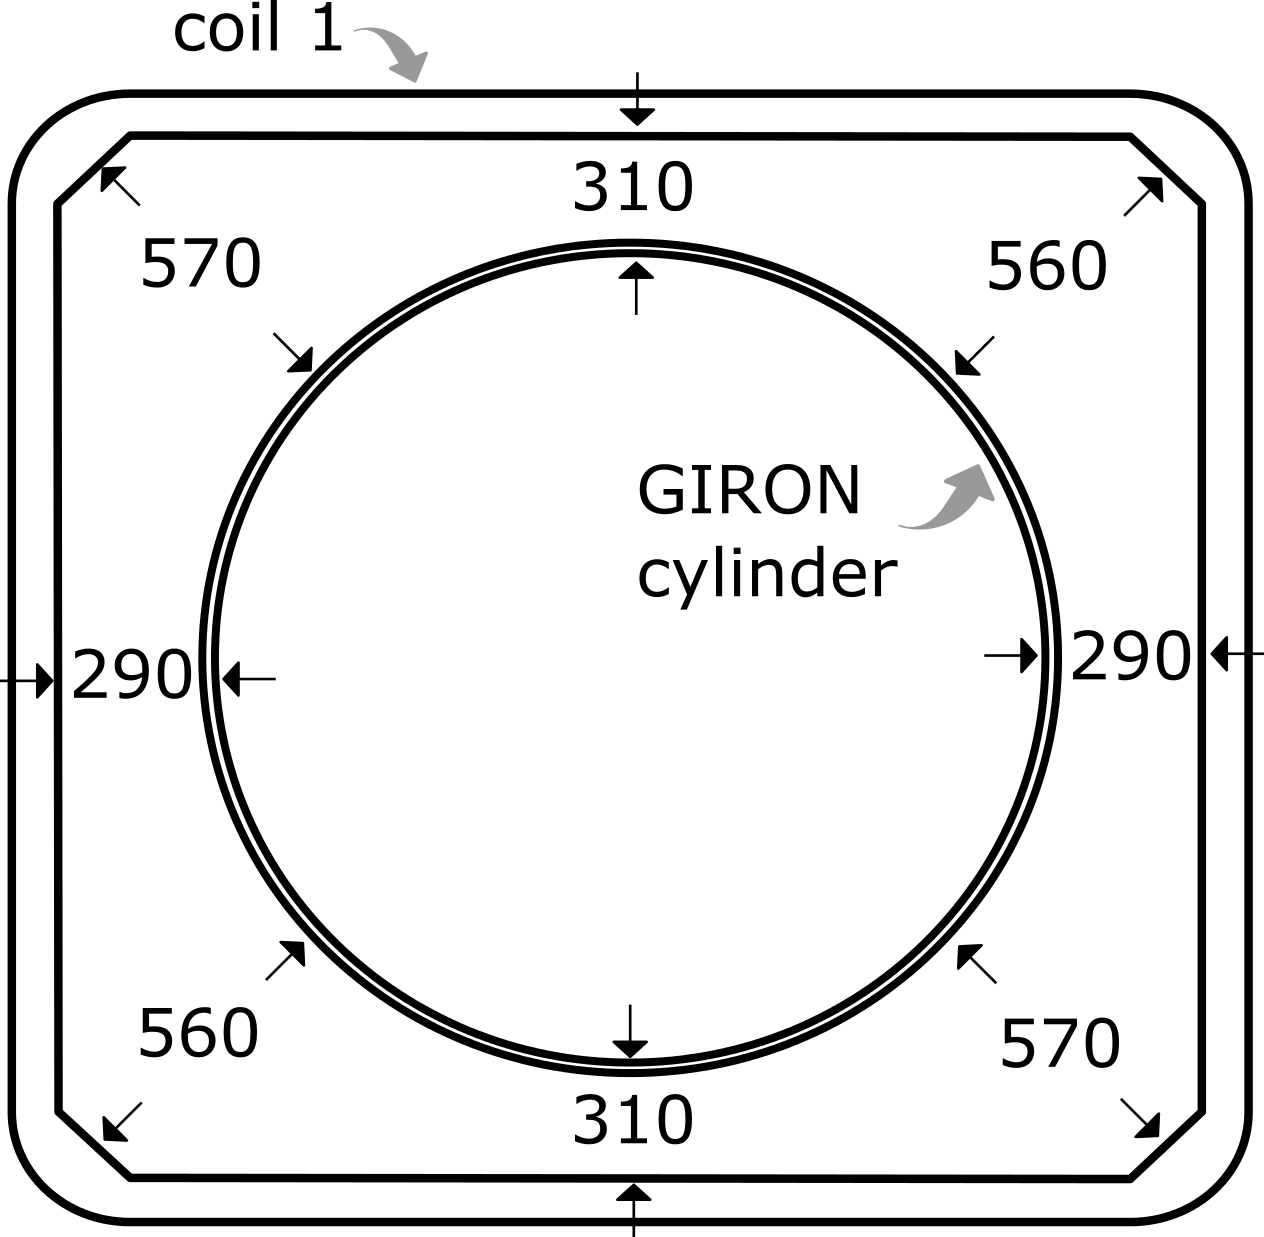
\includegraphics[width=0.4\textwidth]{bfield_PTFGIRONposition.png}
   \caption{Top view of the PTF showing the position of cylindrical GIRON shielding relative to coil 1; dimensions are in millimeters ($\pm2$ mm).}
   \label{fig:gironpos}
   \end{center}
\end{figure}
%
%
\begin{figure}[hp]
   \begin{center}
   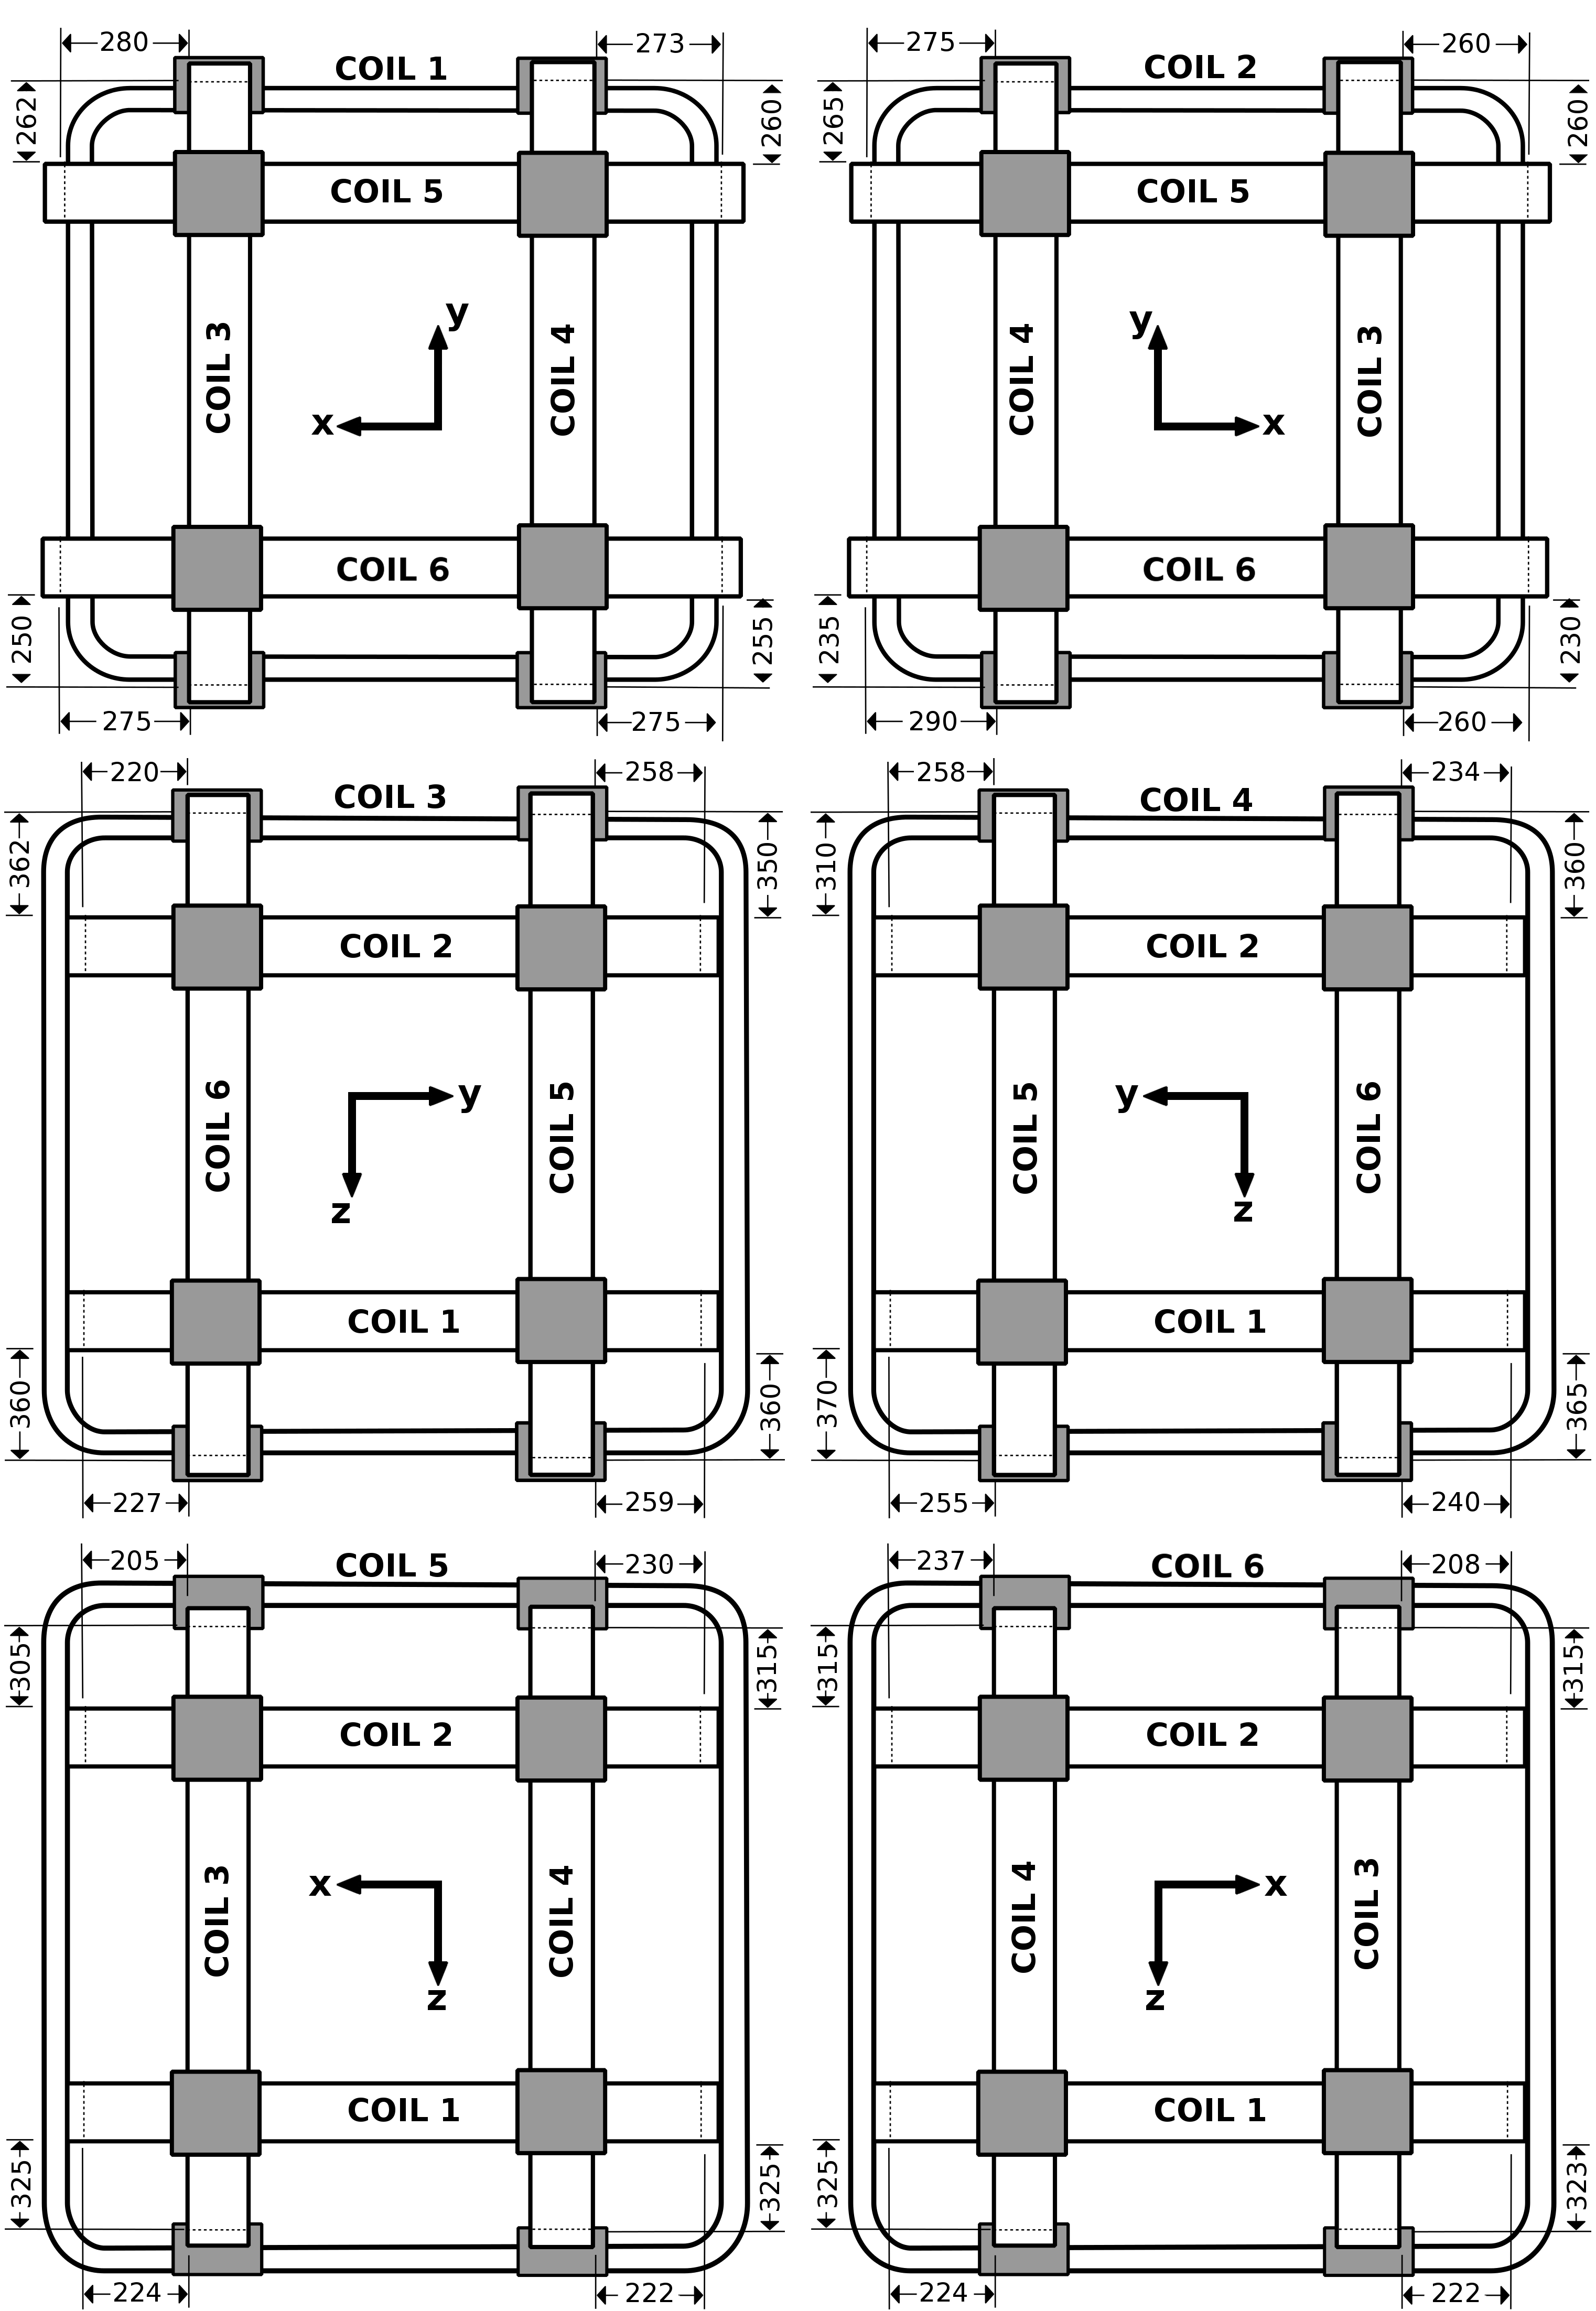
\includegraphics[width=0.8\textwidth]{bfield_PTFcoilpositions.png}
   \caption{PTF compensation coil positions; dimensions are in millimeters ($\pm2$ mm).}
   \label{fig:coilpos}
   \end{center}
\end{figure}

\newpage
\section{Magnetic Field Scan Plots}
\label{Appendix:MagneticFieldScanPlots}

\subsection{Fully Compensated Magnetic Field}
\label{Appendix:PlotsofFullCompensation}

The following plots show magnetic field maps in the x-y plane at different heights for when the magnetic field in the PTF is fully compensated, so that the center of the scan volume has a magnetic field of zero magnitude. The first three pages are plots of full compensation when the main magnets of TRIUMF's cyclotron are turned off, and the three pages that follow are plots of full compensation when the cyclotron magnets are turned on. 

%
\begin{figure}[h!]
  \begin{center}
    \subfloat[Magnetic field magnitude and vector field\label{fig:bfield_fullcomp500_vec_cycloOFF}]{
      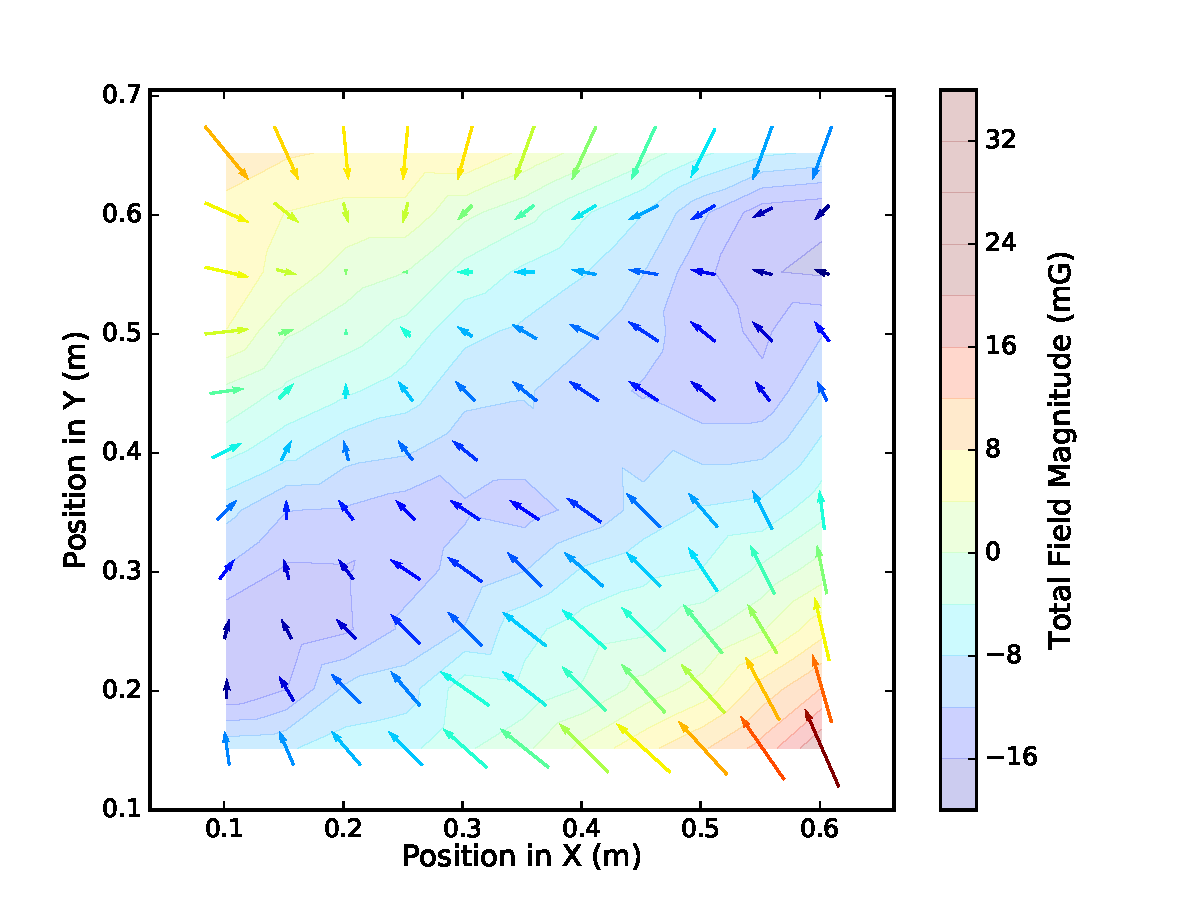
\includegraphics[width=0.5\textwidth]{bfield_full_compensation_cycloOFF2_z500_vec.pdf}
    }
    \subfloat[x-component of magnetic field\label{fig:bfield_fullcomp500_x_cycloOFF}]{
      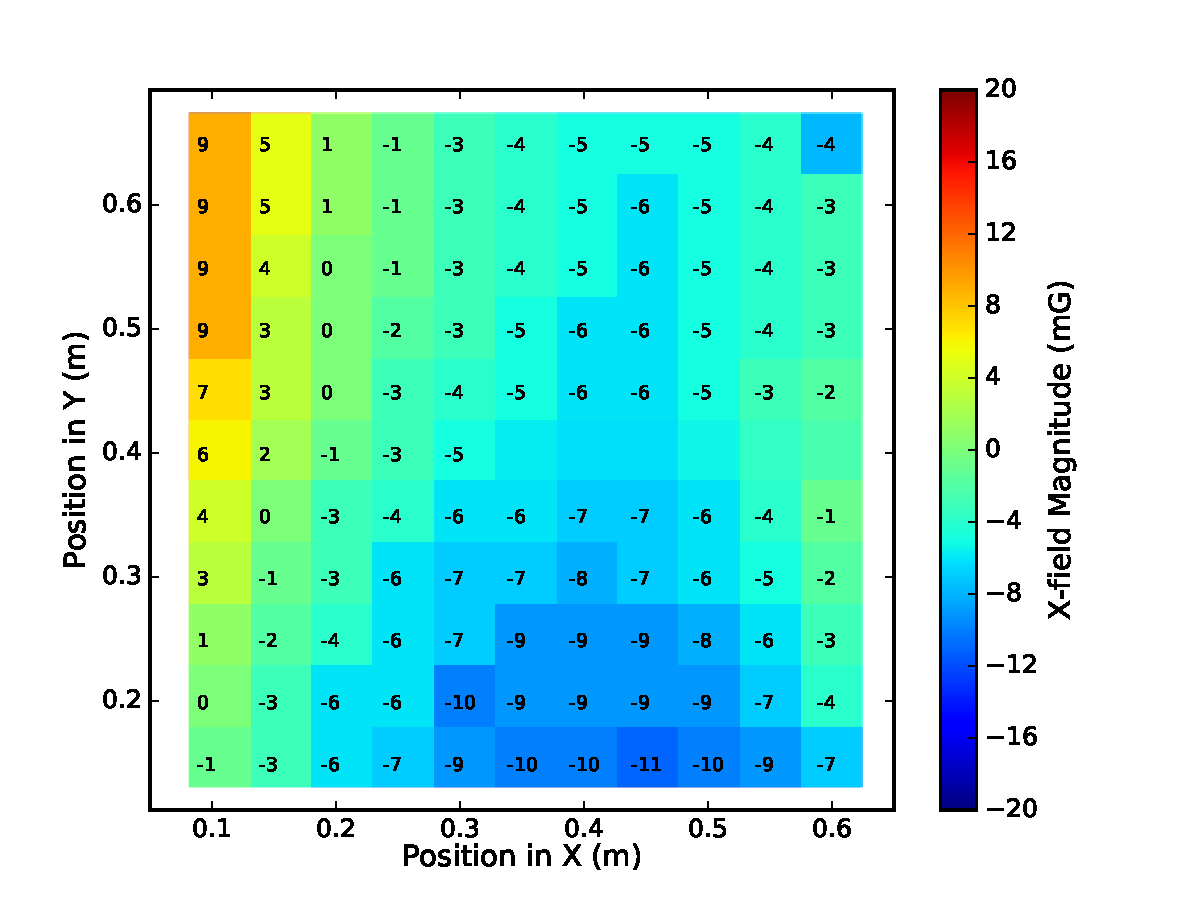
\includegraphics[width=0.5\textwidth]{bfield_full_compensation_cycloOFF2_z500_x.pdf}
    }\\
    \vspace{-3 mm}
    \subfloat[y-component of magnetic field\label{fig:bfield_fullcomp500_y_cycloOFF}]{
      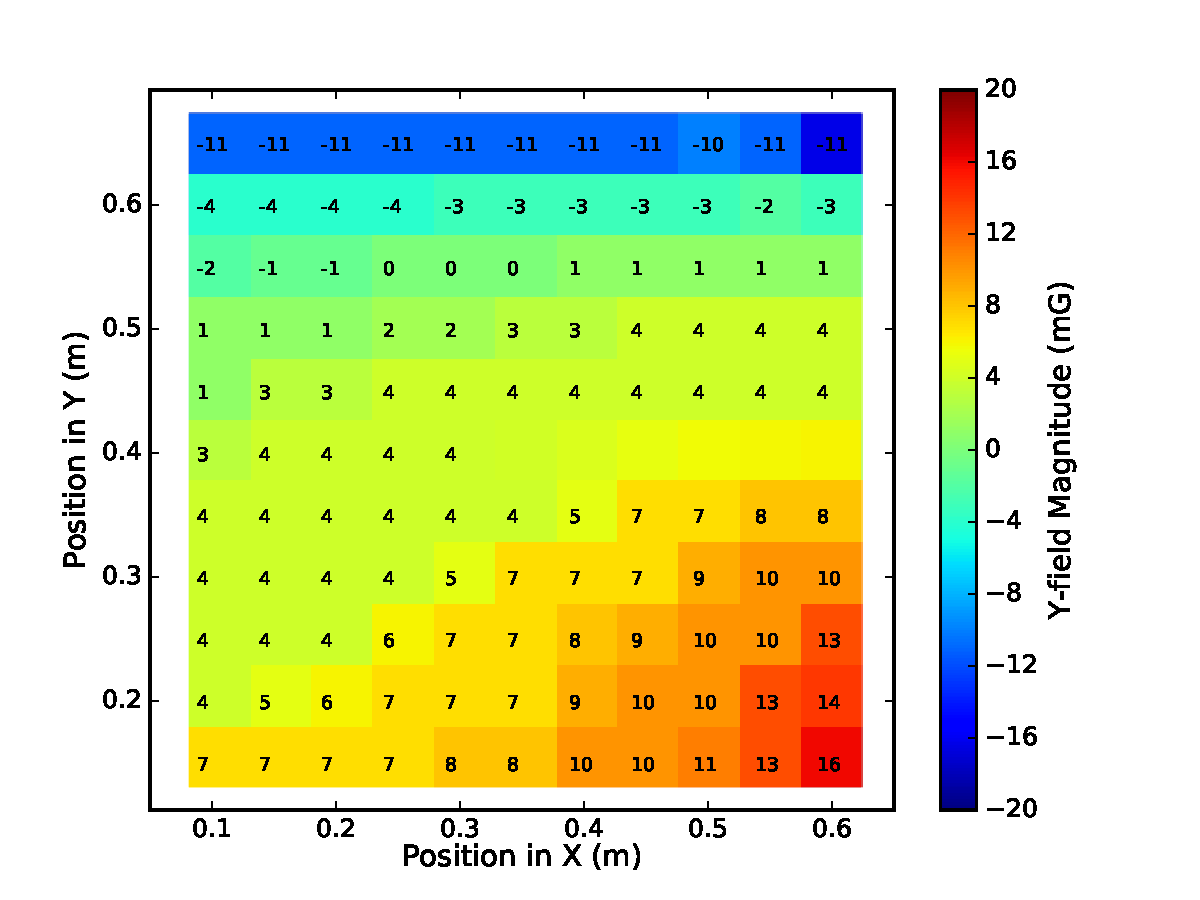
\includegraphics[width=0.5\textwidth]{bfield_full_compensation_cycloOFF2_z500_y.pdf}
    }
    \subfloat[z-component of magnetic field\label{fig:bfield_fullcomp500_z_cycloOFF}]{
      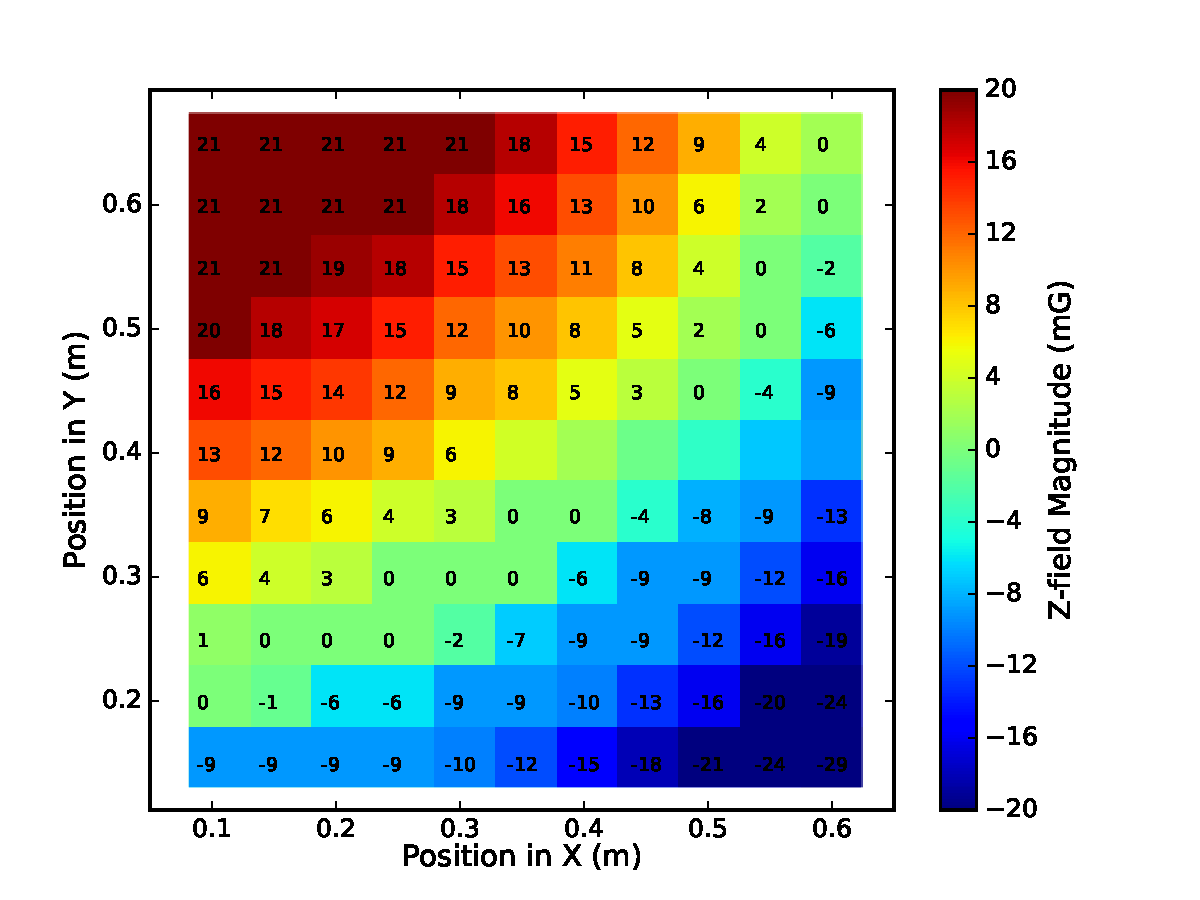
\includegraphics[width=0.5\textwidth]{bfield_full_compensation_cycloOFF2_z500_z.pdf}
    }
  \caption{Plots of fully compensated magnetic field with the cyclotron off, in the x-y plane at a height just above the top of the PMT.}
  \label{fig:bfield_fullcomp500_cycloOFF}
  \end{center}
\end{figure}
%
%
\begin{figure}[hp]
  \begin{center}
    \subfloat[Magnetic field magnitude and vector field\label{fig:bfield_fullcomp700_vec_cycloOFF}]{
      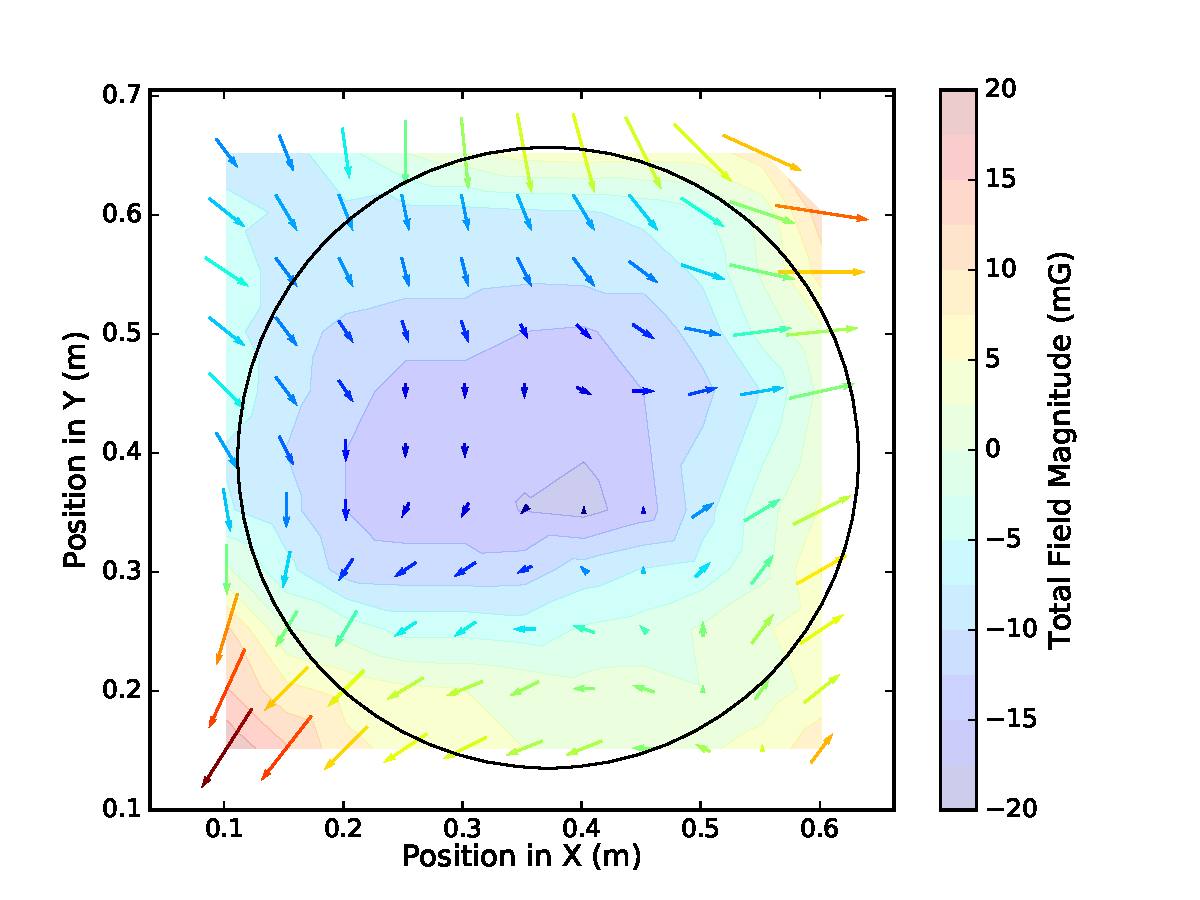
\includegraphics[width=0.5\textwidth]{bfield_full_compensation_cycloOFF2_z700_vec.pdf}
    }
    \subfloat[x-component of magnetic field\label{fig:bfield_fullcomp700_x_cycloOFF}]{
      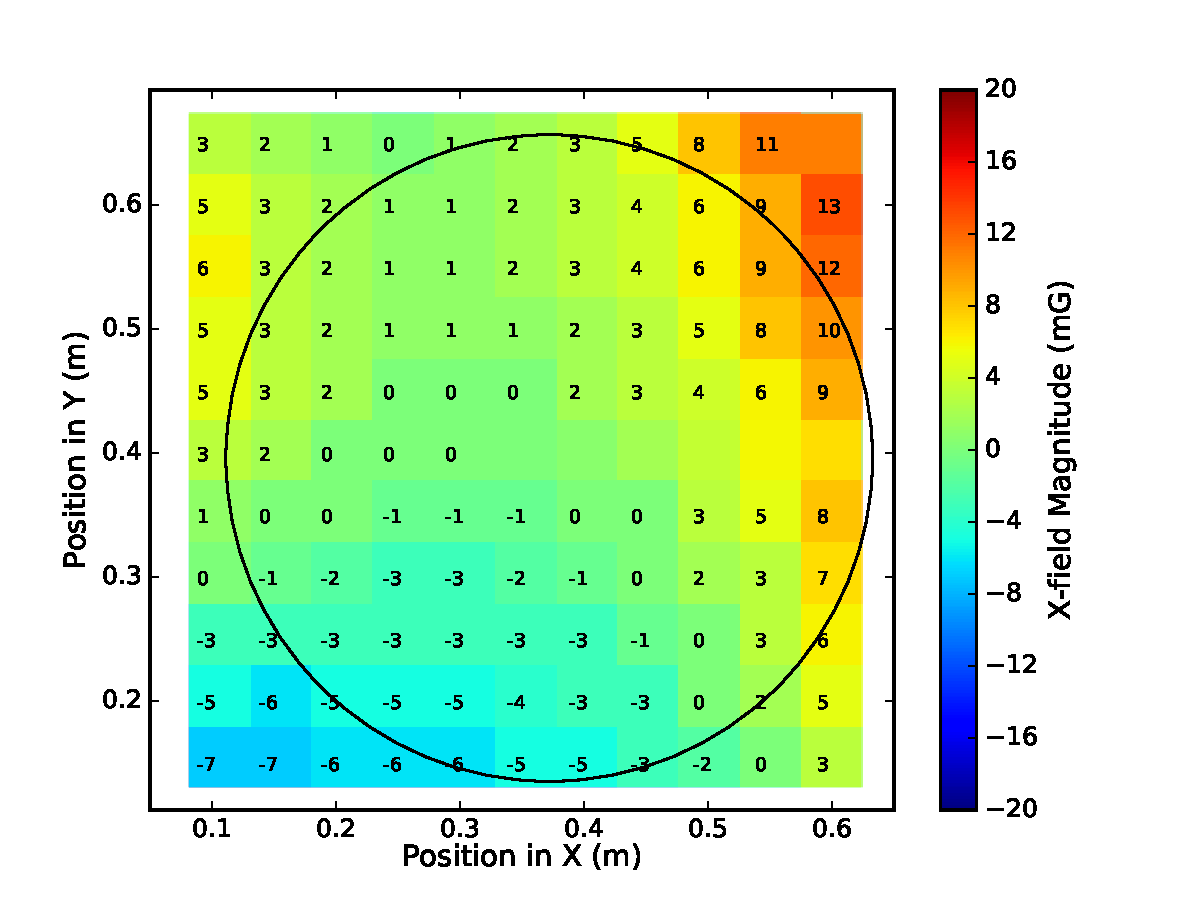
\includegraphics[width=0.5\textwidth]{bfield_full_compensation_cycloOFF2_z700_x.pdf}
    }\\
    \vspace{-3 mm}
    \subfloat[y-component of magnetic field\label{fig:bfield_fullcomp700_y_cycloOFF}]{
      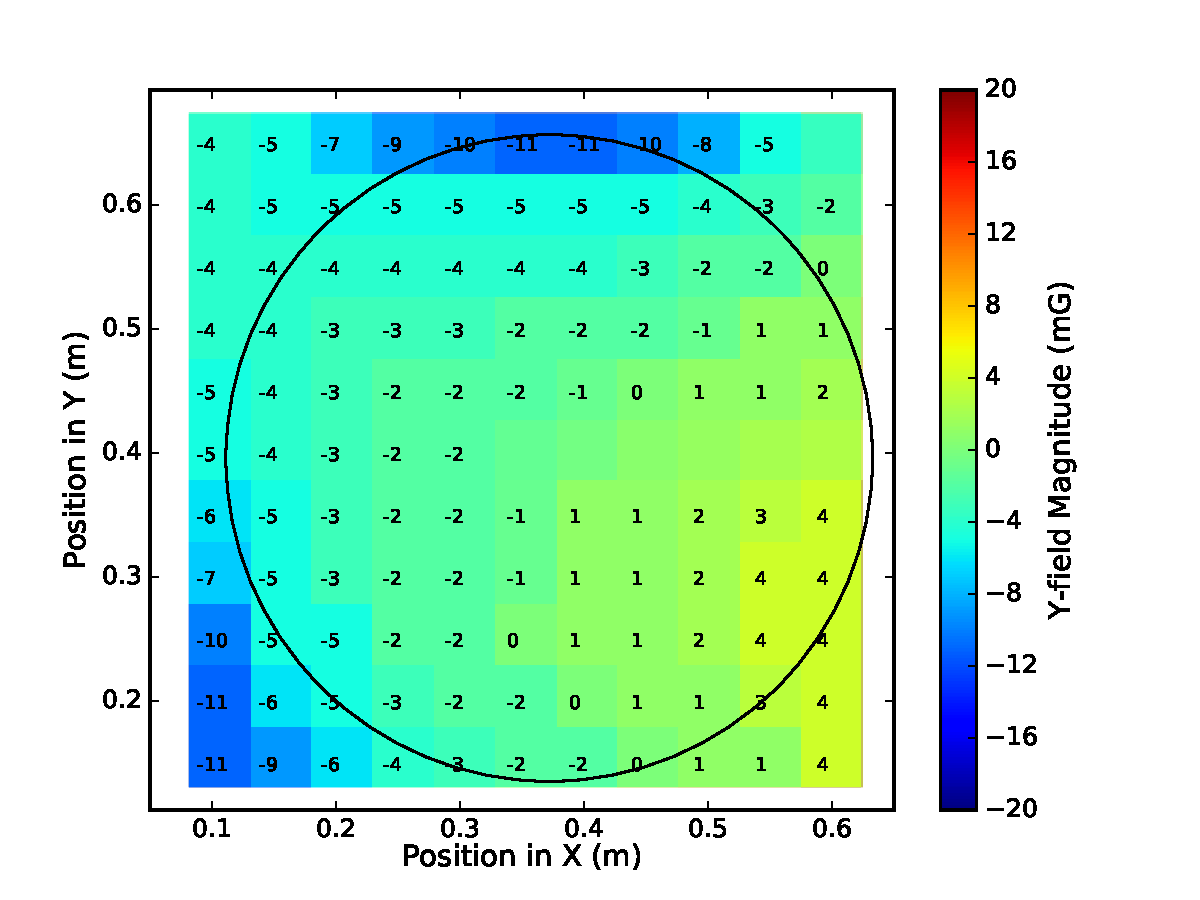
\includegraphics[width=0.5\textwidth]{bfield_full_compensation_cycloOFF2_z700_y.pdf}
    }
    \subfloat[z-component of magnetic field\label{fig:bfield_fullcomp700_z_cycloOFF}]{
      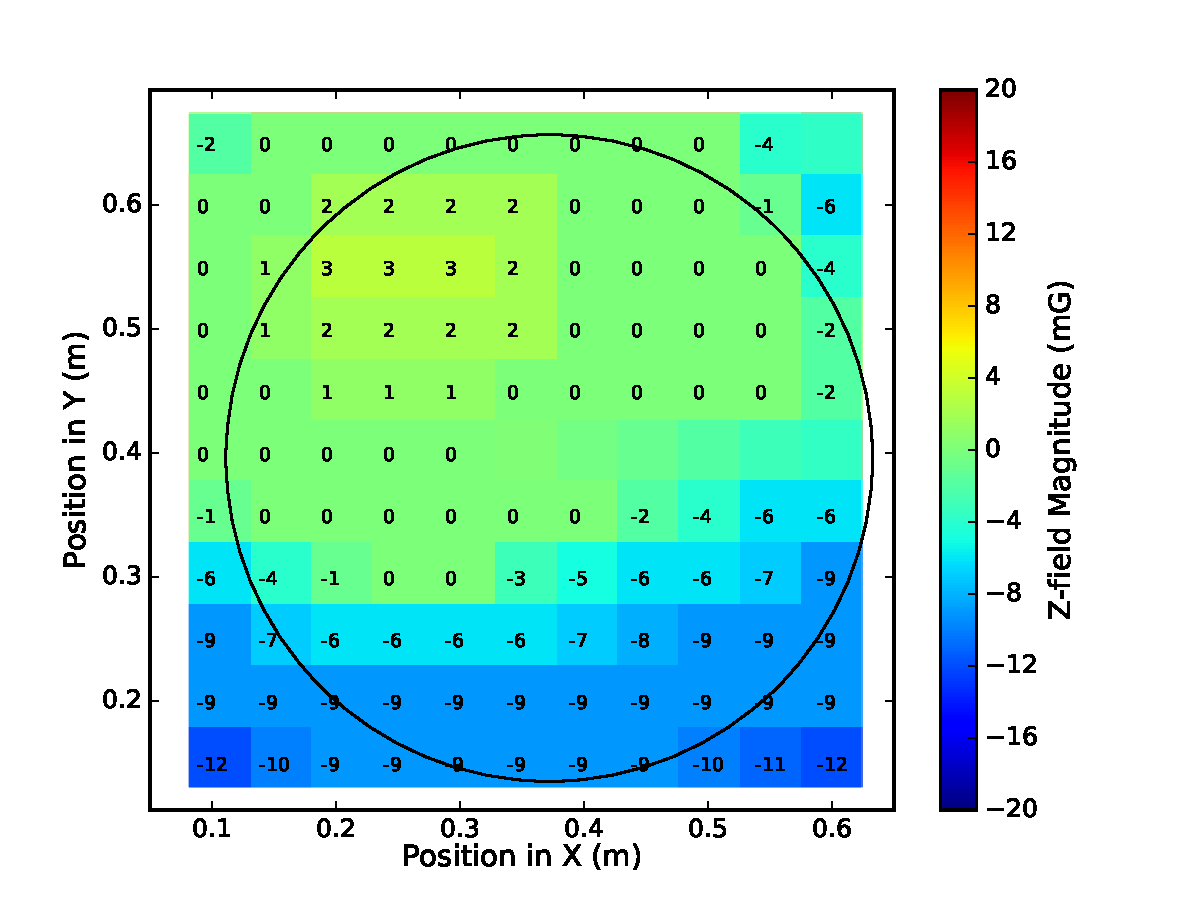
\includegraphics[width=0.5\textwidth]{bfield_full_compensation_cycloOFF2_z700_z.pdf}
    }
  \caption{Plots of fully compensated magnetic field with the cyclotron off, in the x-y plane at the height of the center of the 20'' PMT's electron-path trajectory.}
  \label{fig:bfield_fullcomp700_cycloOFF}
  \end{center}
\end{figure}
%
%
\begin{figure}[hp]
  \begin{center}
    \subfloat[Magnetic field magnitude and vector field\label{fig:bfield_fullcomp900_vec_cycloOFF}]{
      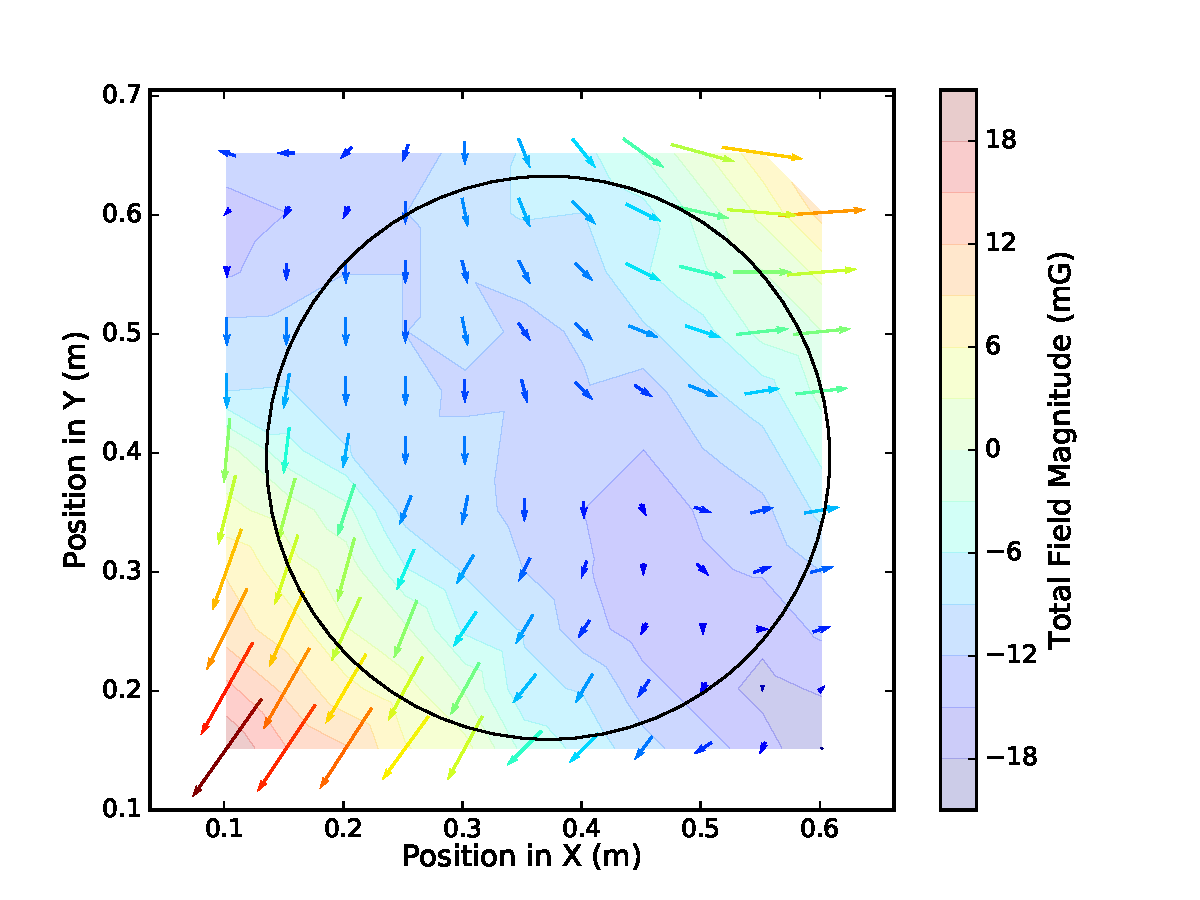
\includegraphics[width=0.5\textwidth]{bfield_full_compensation_cycloOFF2_z900_vec.pdf}
    }
    \subfloat[x-component of magnetic field\label{fig:bfield_fullcomp900_x_cycloOFF}]{
      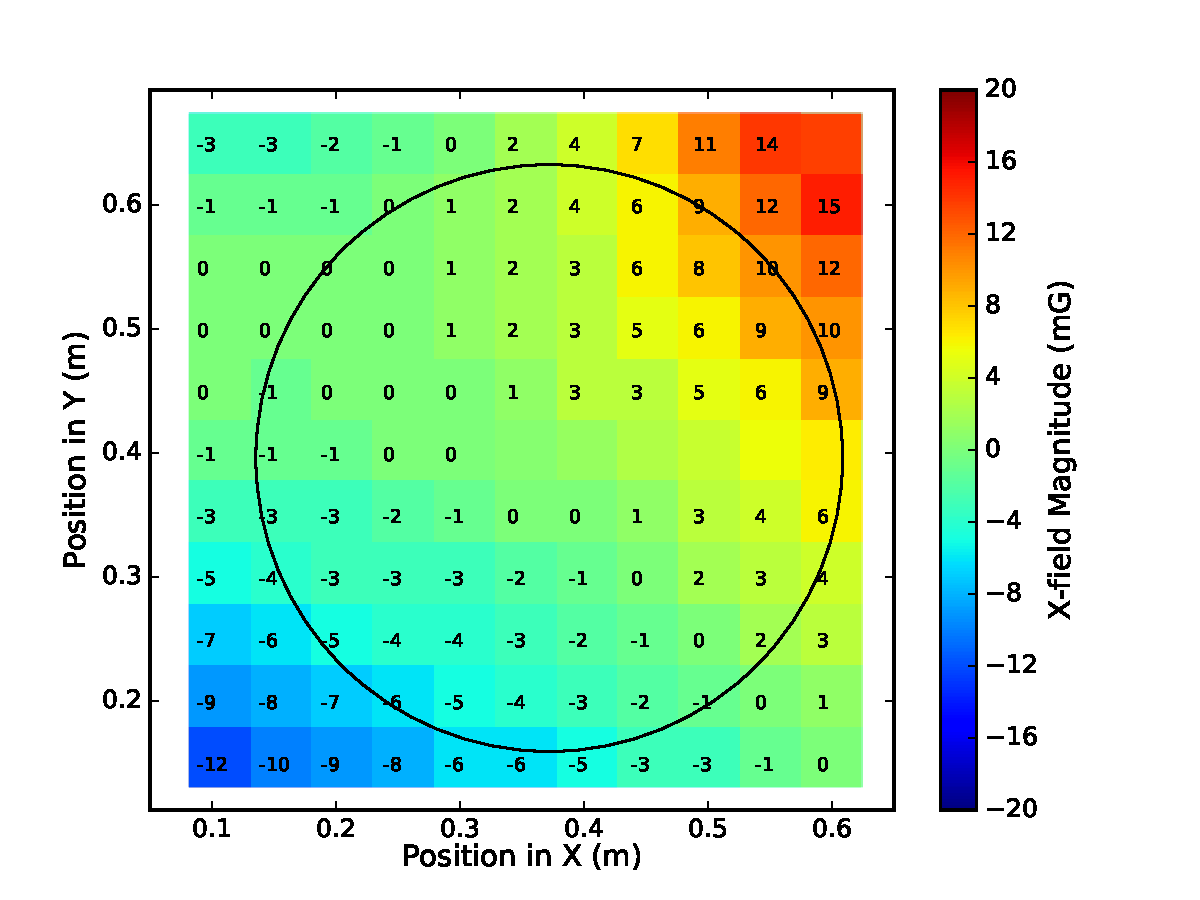
\includegraphics[width=0.5\textwidth]{bfield_full_compensation_cycloOFF2_z900_x.pdf}
    }\\
    \vspace{-3 mm}
    \subfloat[y-component of magnetic field\label{fig:bfield_fullcomp900_y_cycloOFF}]{
      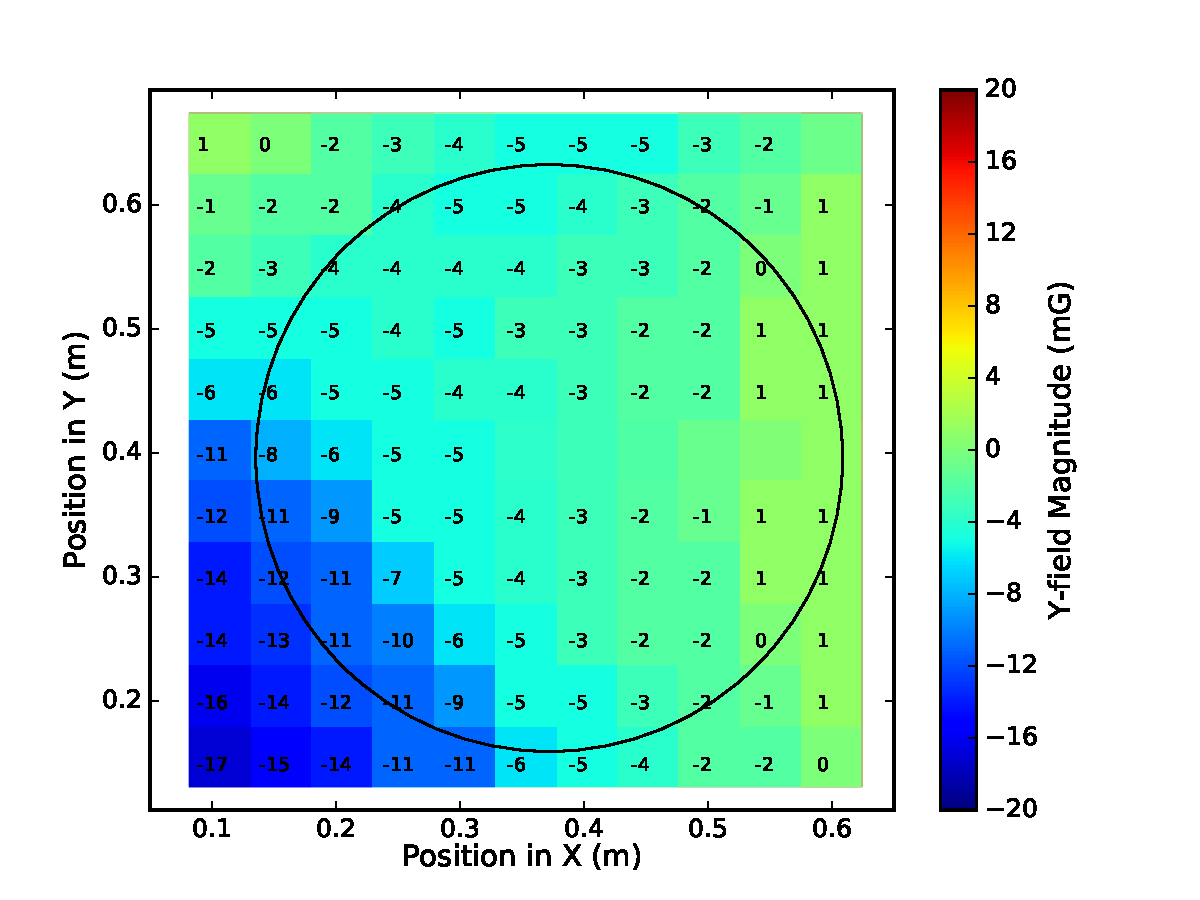
\includegraphics[width=0.5\textwidth]{bfield_full_compensation_cycloOFF2_z900_y.pdf}
    }
    \subfloat[z-component of magnetic field\label{fig:bfield_fullcomp900_z_cycloOFF}]{
      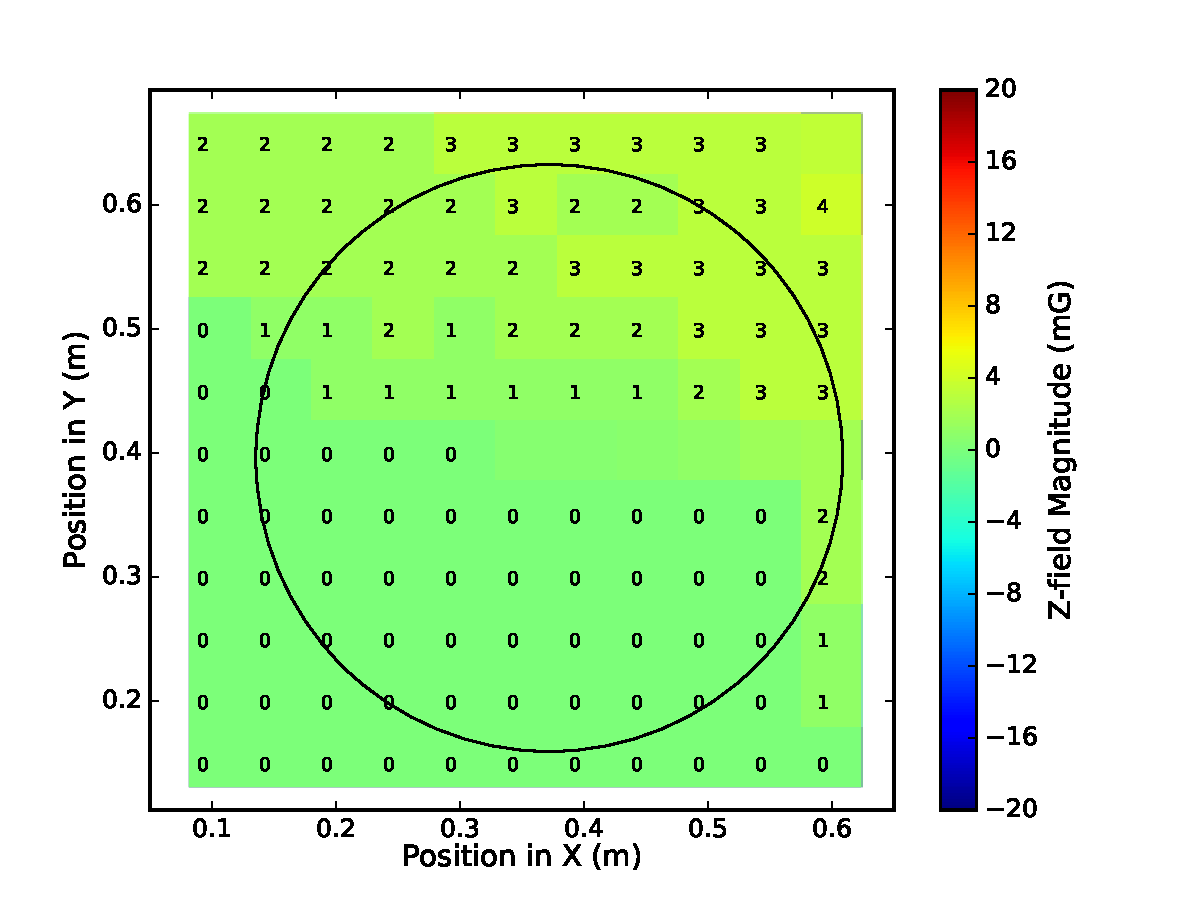
\includegraphics[width=0.5\textwidth]{bfield_full_compensation_cycloOFF2_z900_z.pdf}
    }
  \caption{Plots of fully compensated magnetic field with the cyclotron off, in the x-y plane at the height of the first dynode of the 20'' PMT.}
  \label{fig:bfield_fullcomp900_cycloOFF}
  \end{center}
\end{figure}
%
%
\begin{figure}[hp]
  \begin{center}
    \subfloat[Magnetic field magnitude and vector field\label{fig:bfield_fullcomp400_vec}]{
      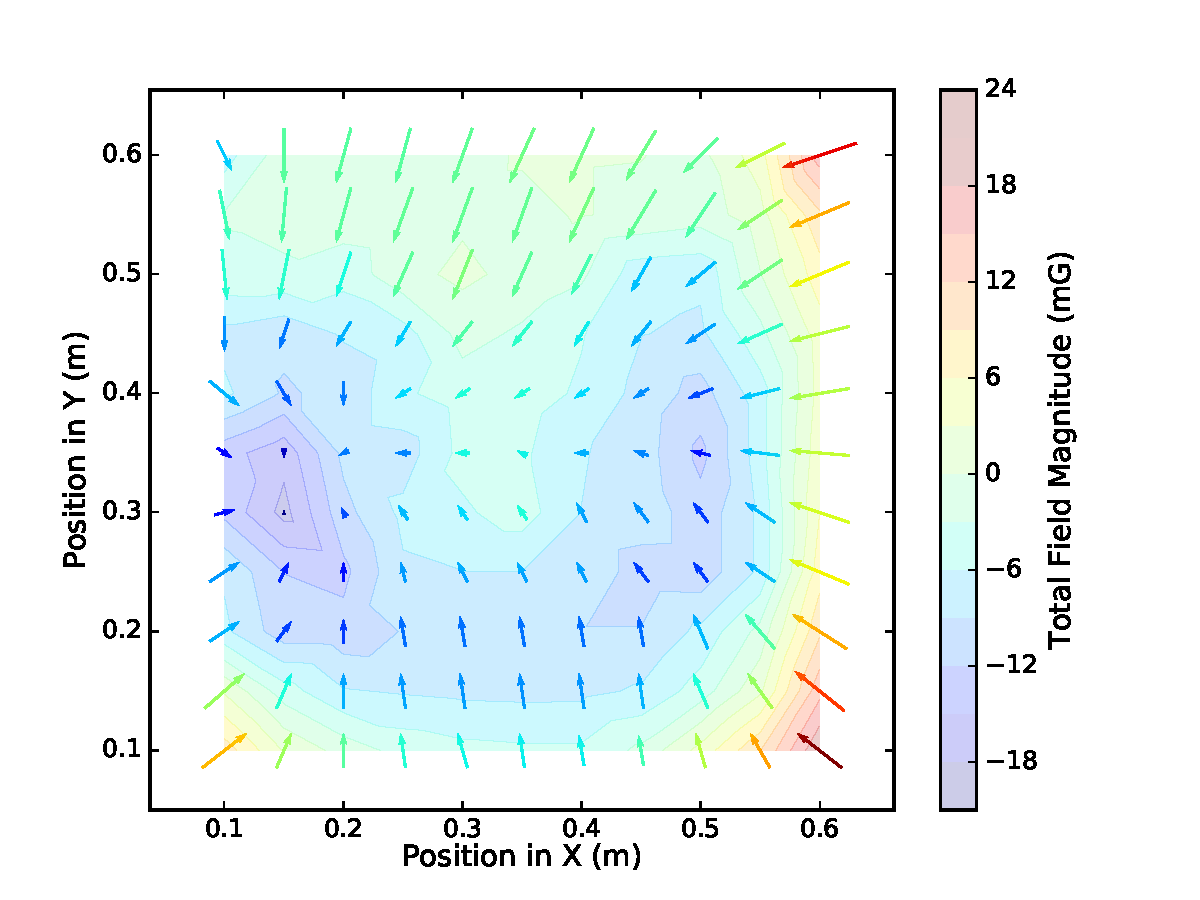
\includegraphics[width=0.5\textwidth]{bfield_full_compensation_z400_vec.pdf}
    }
    \subfloat[x-component of magnetic field\label{fig:bfield_fullcomp400_x}]{
      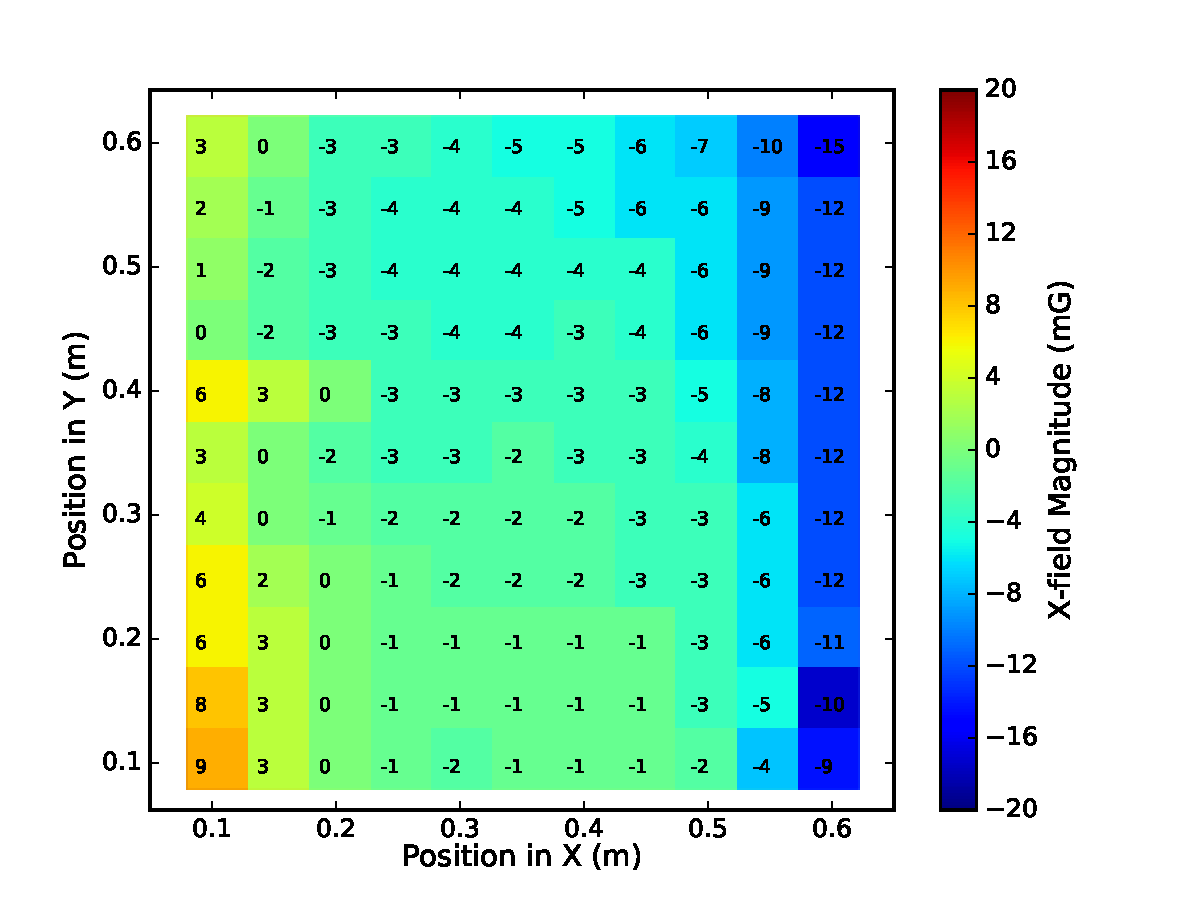
\includegraphics[width=0.5\textwidth]{bfield_full_compensation_z400_x.pdf}
    }\\
    \vspace{-3 mm}
    \subfloat[y-component of magnetic field\label{fig:bfield_fullcomp400_y}]{
      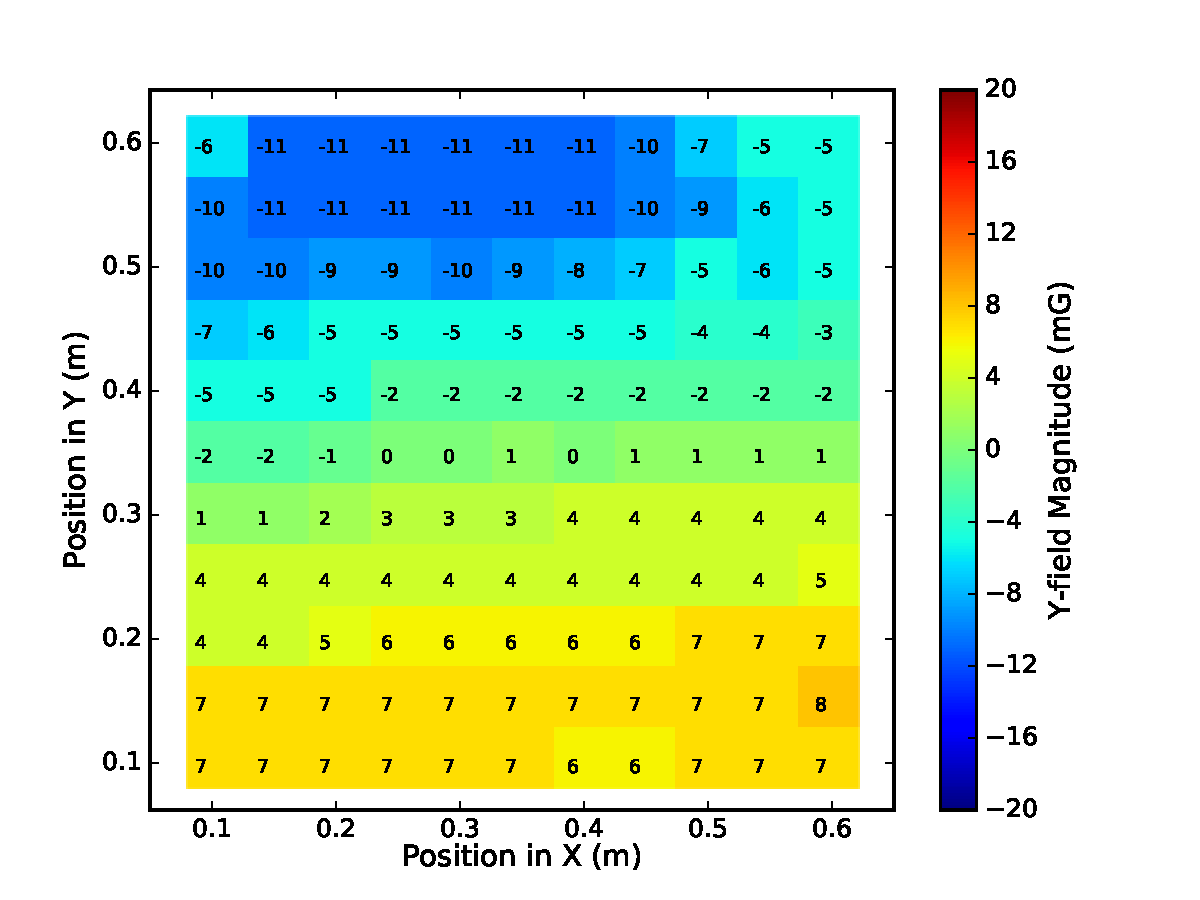
\includegraphics[width=0.5\textwidth]{bfield_full_compensation_z400_y.pdf}
    }
    \subfloat[z-component of magnetic field\label{fig:bfield_fullcomp400_z}]{
      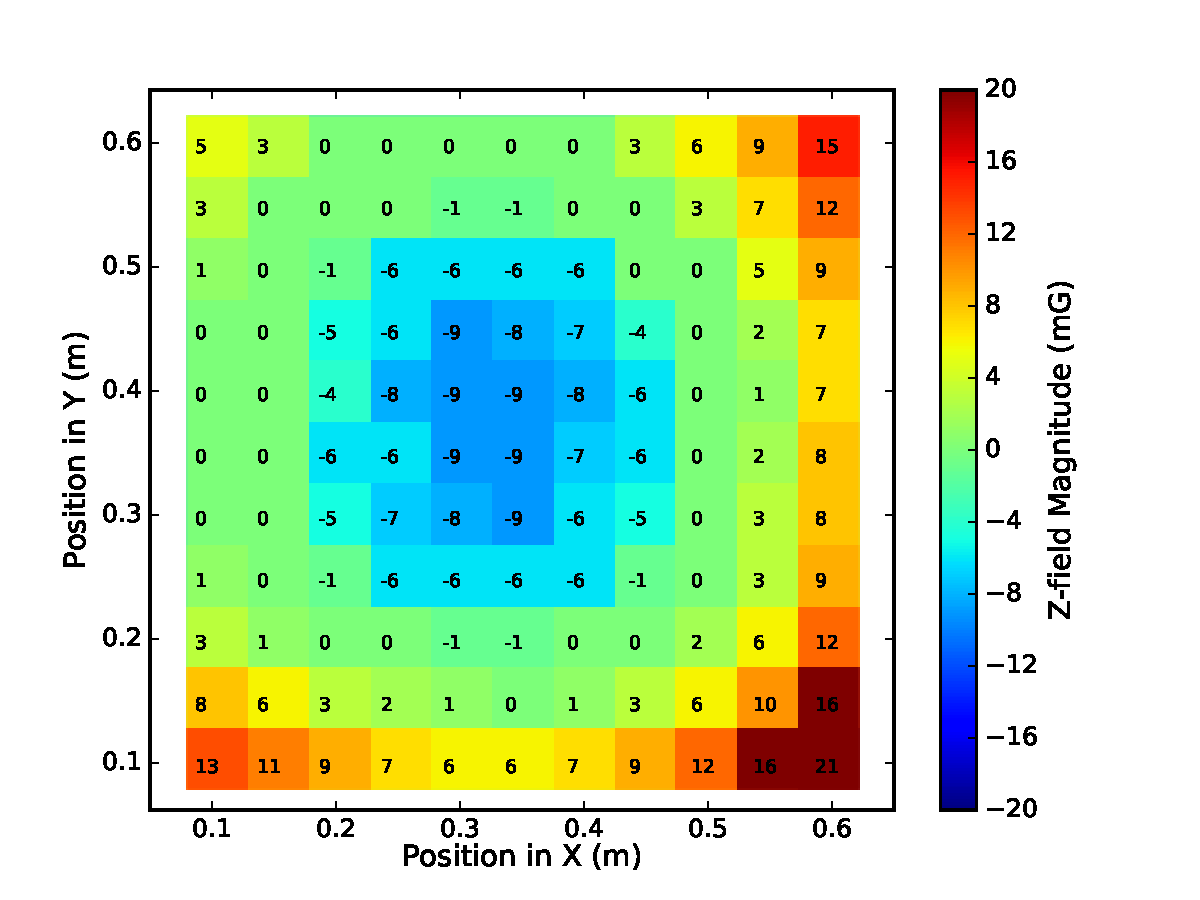
\includegraphics[width=0.5\textwidth]{bfield_full_compensation_z400_z.pdf}
    }
  \caption{Plots of fully compensated magnetic field with the cyclotron on, in the x-y plane at a height just above the top of the PMT.}
  \label{fig:bfield_fullcomp400}
  \end{center}
\end{figure}
%
%
\begin{figure}[hp]
  \begin{center}
    \subfloat[Magnetic field magnitude and vector field\label{fig:bfield_fullcomp600_vec}]{
      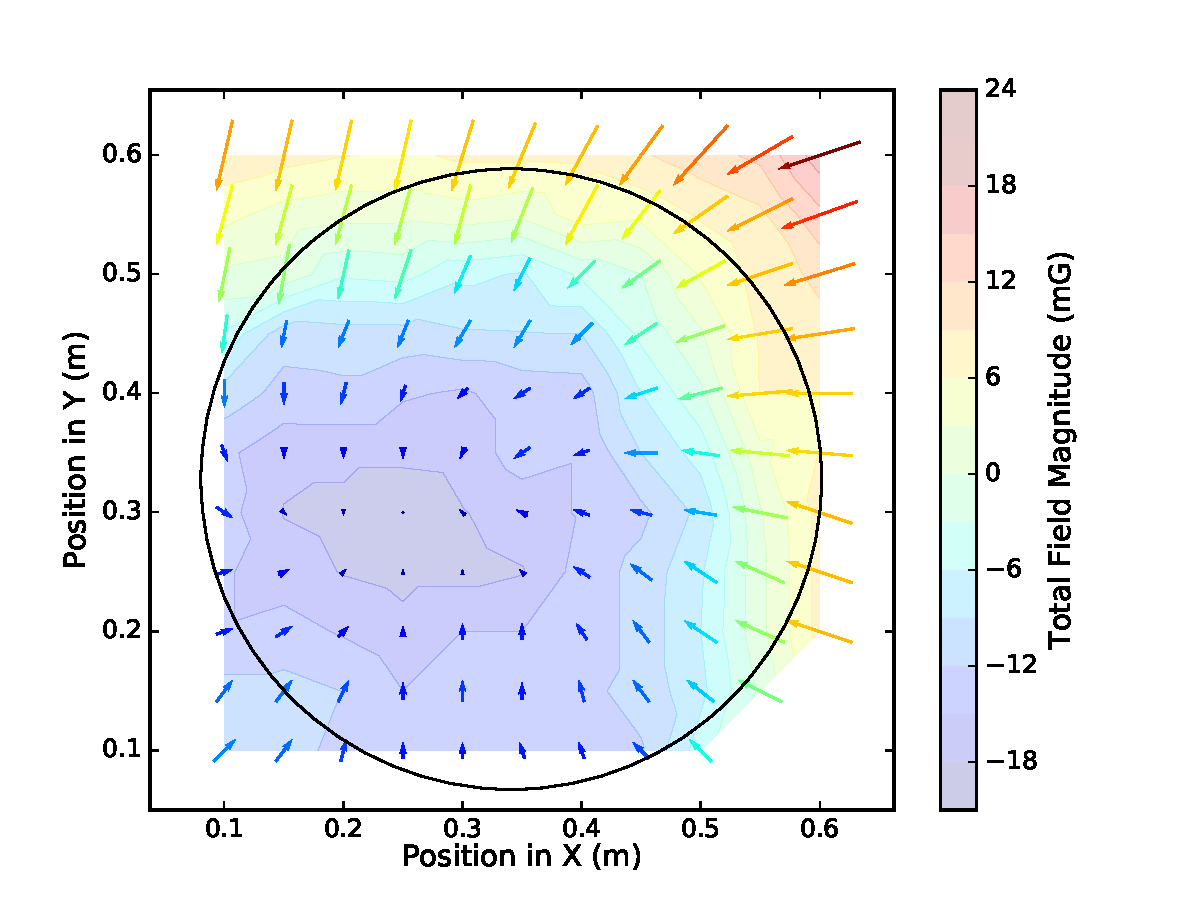
\includegraphics[width=0.5\textwidth]{bfield_full_compensation_z600_vec.pdf}
    }
    \subfloat[x-component of magnetic field\label{fig:bfield_fullcomp600_x}]{
      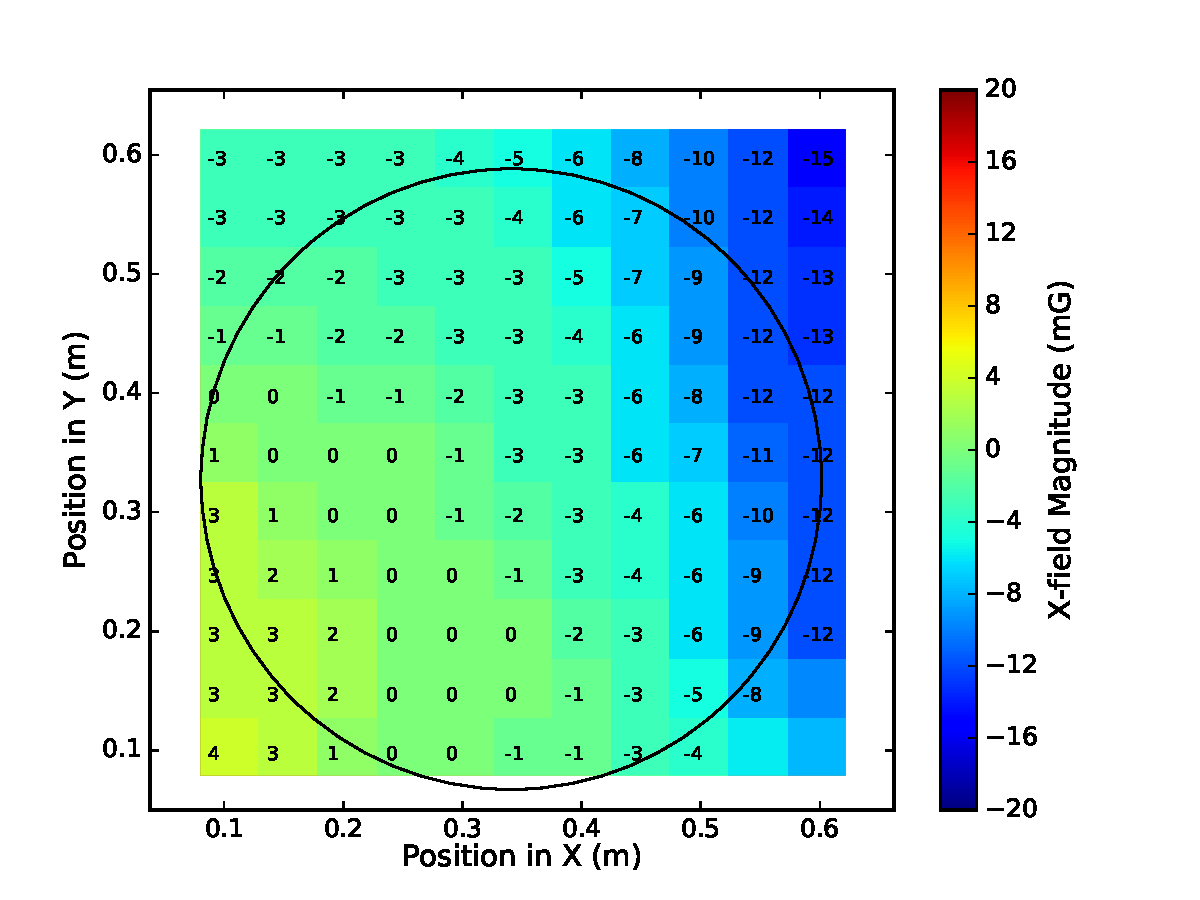
\includegraphics[width=0.5\textwidth]{bfield_full_compensation_z600_x.pdf}
    }\\
    \vspace{-3 mm}
    \subfloat[y-component of magnetic field\label{fig:bfield_fullcomp600_y}]{
      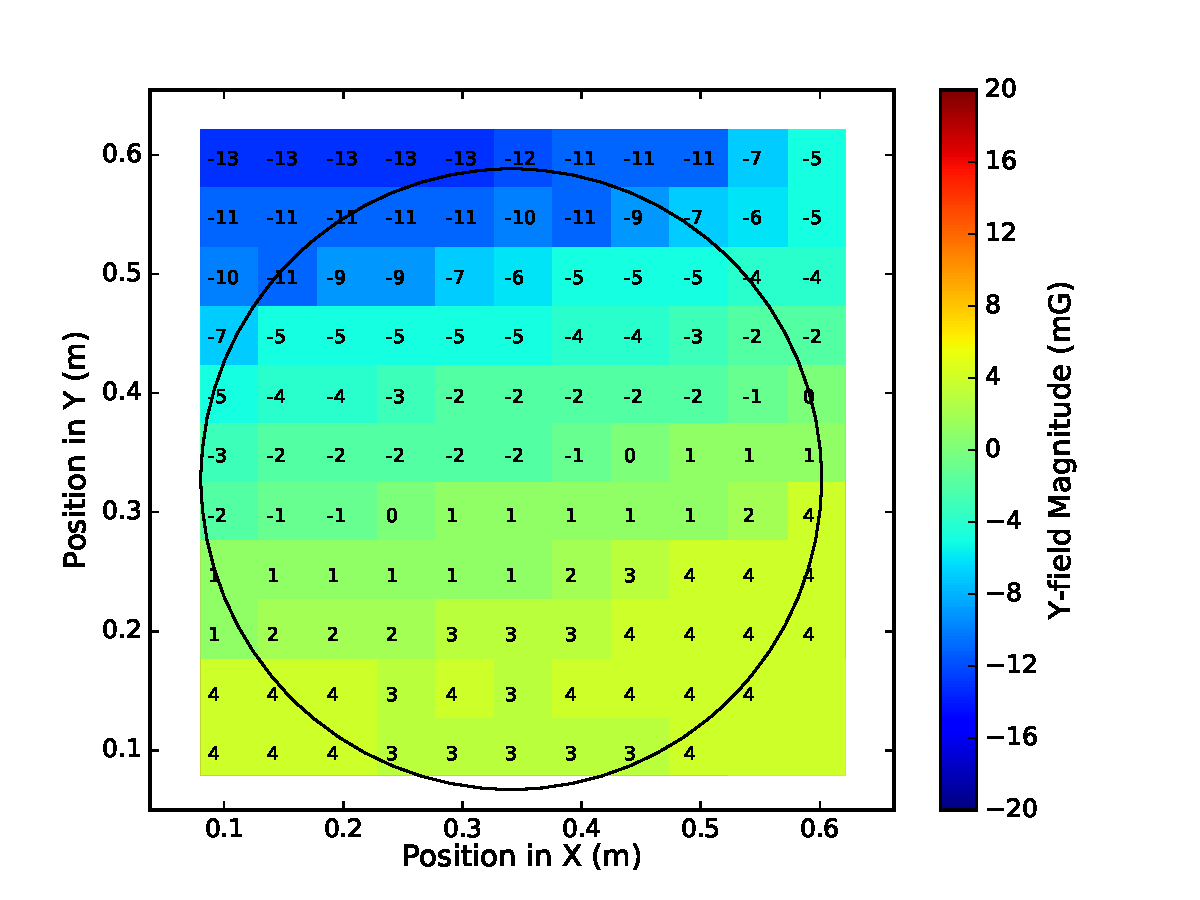
\includegraphics[width=0.5\textwidth]{bfield_full_compensation_z600_y.pdf}
    }
    \subfloat[z-component of magnetic field\label{fig:bfield_fullcomp600_z}]{
      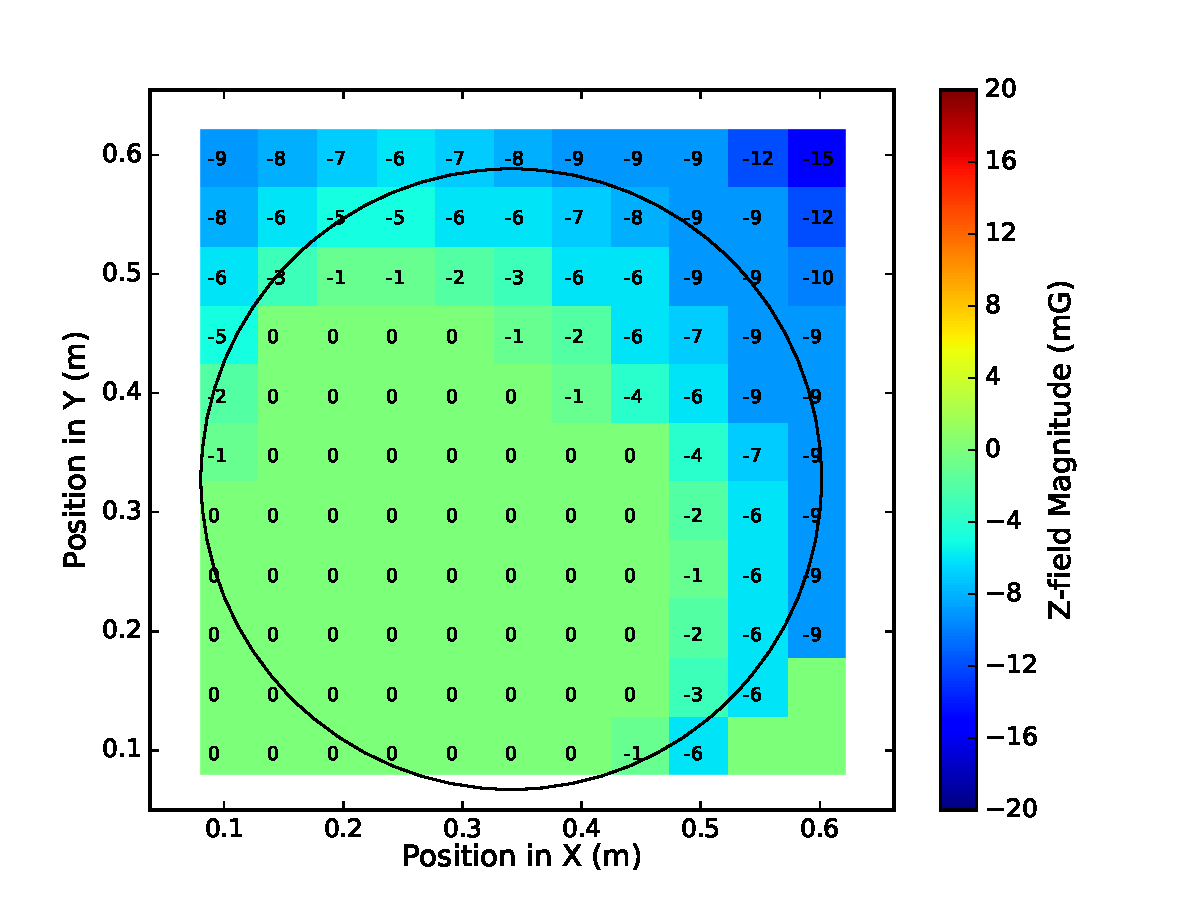
\includegraphics[width=0.5\textwidth]{bfield_full_compensation_z600_z.pdf}
    }
  \caption{Plots of fully compensated magnetic field with the cyclotron on, in the x-y plane at the height of the center of the 20'' PMT's electron-path trajectory.}
  \label{fig:bfield_fullcomp600}
  \end{center}
\end{figure}
%
%
\begin{figure}[hp]
  \begin{center}
    \subfloat[Magnetic field magnitude and vector field\label{fig:bfield_fullcomp800_vec}]{
      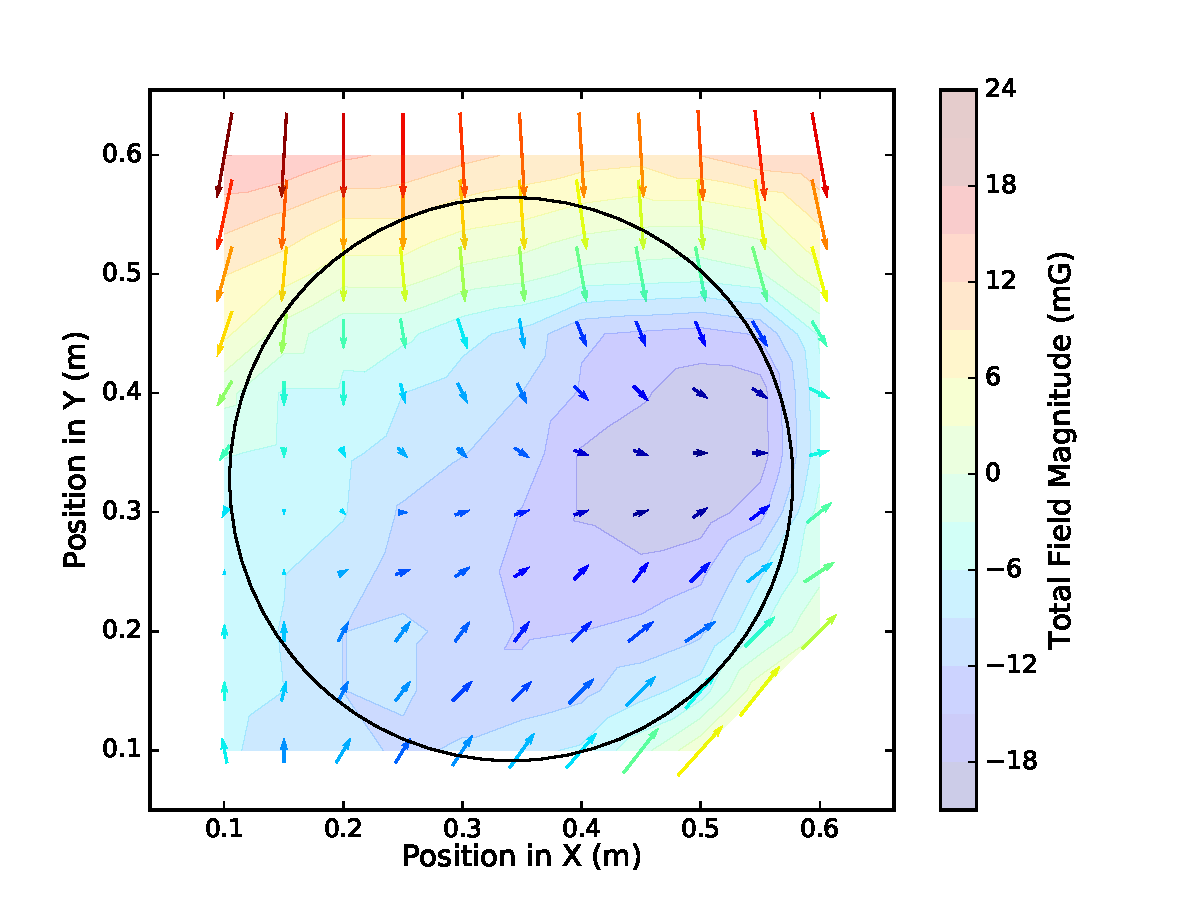
\includegraphics[width=0.5\textwidth]{bfield_full_compensation_z800_vec.pdf}
    }
    \subfloat[x-component of magnetic field\label{fig:bfield_fullcomp800_x}]{
      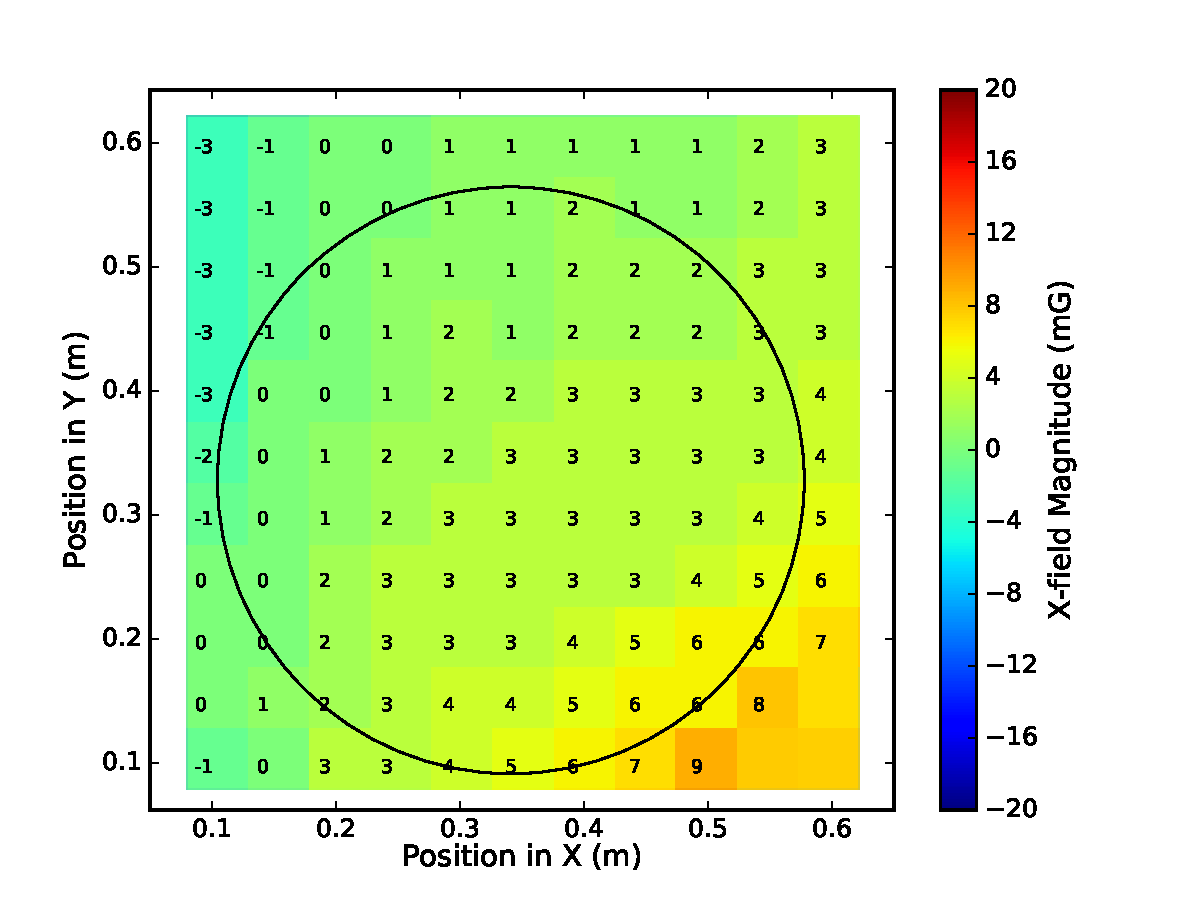
\includegraphics[width=0.5\textwidth]{bfield_full_compensation_z800_x.pdf}
    }\\
    \vspace{-3 mm}
    \subfloat[y-component of magnetic field\label{fig:bfield_fullcomp800_y}]{
      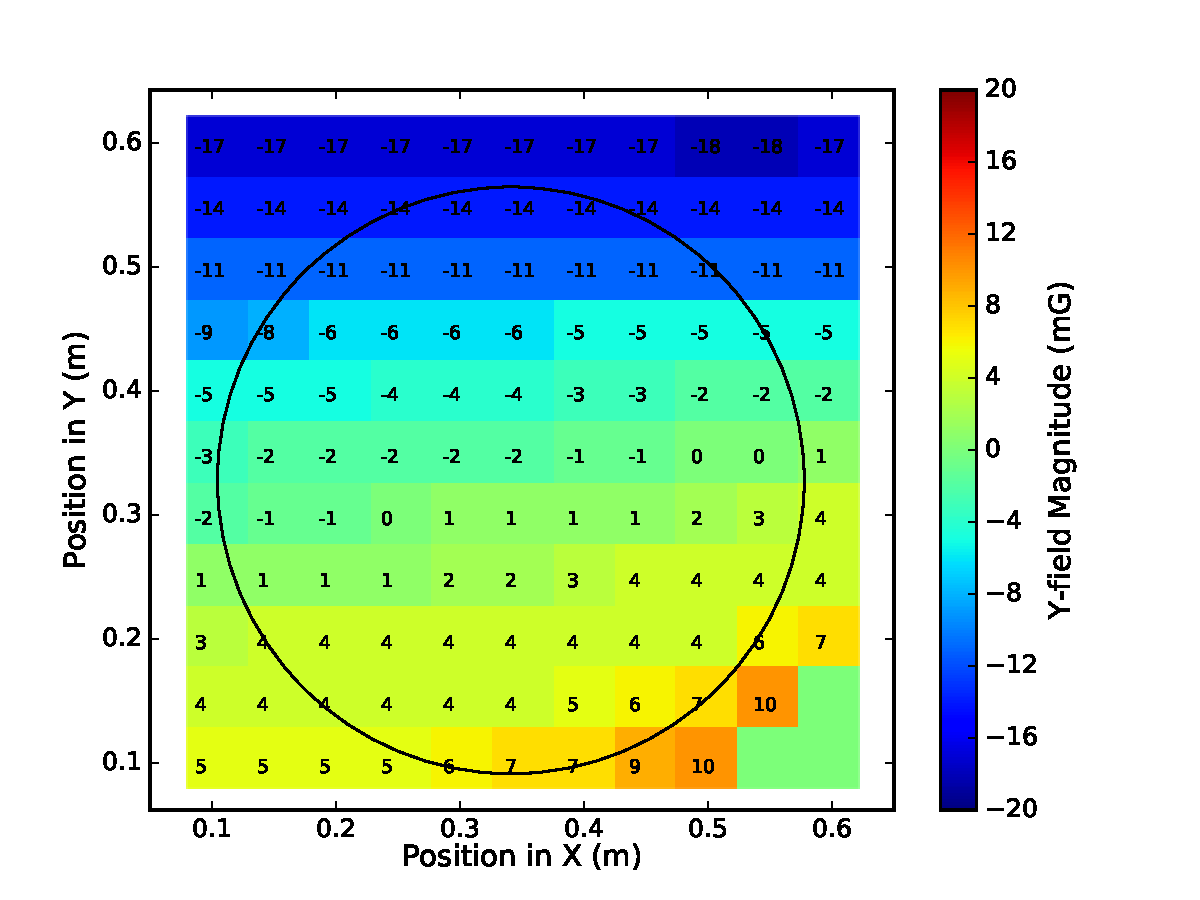
\includegraphics[width=0.5\textwidth]{bfield_full_compensation_z800_y.pdf}
    }
    \subfloat[z-component of magnetic field\label{fig:bfield_fullcomp800_z}]{
      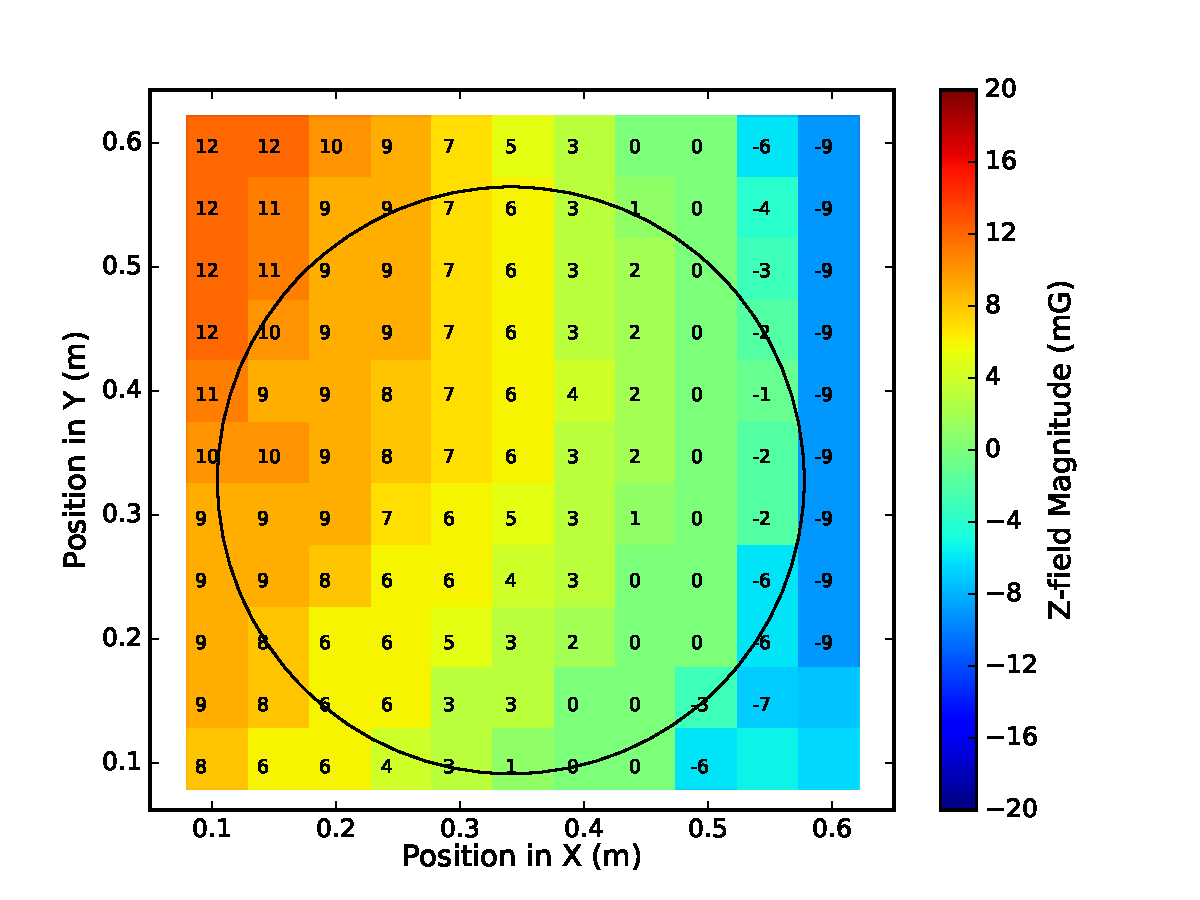
\includegraphics[width=0.5\textwidth]{bfield_full_compensation_z800_z.pdf}
    }
  \caption{Plots of fully compensated magnetic field with the cyclotron on, in the x-y plane at the height of the first dynode of the 20'' PMT.}
  \label{fig:bfield_fullcomp800}
  \end{center}
\end{figure}
%

\newpage
\subsection{Reproducibility Test}
\label{Appendix:ReproducibilityTest}

The following magnetic field maps show the accuracy to which the magnetic fields can be controlled, and the reproducibility of different magnetic field conditions.
All plots show the magnetic fields mapped in the x-y plane at the height of the center of the electron path trajectory.

%
\begin{figure}[h!]
  \begin{center}
    \subfloat[Trial 1: magnetic field magnitude and vector field\label{fig:bfield_rep_Bx50_1_vec}]{
      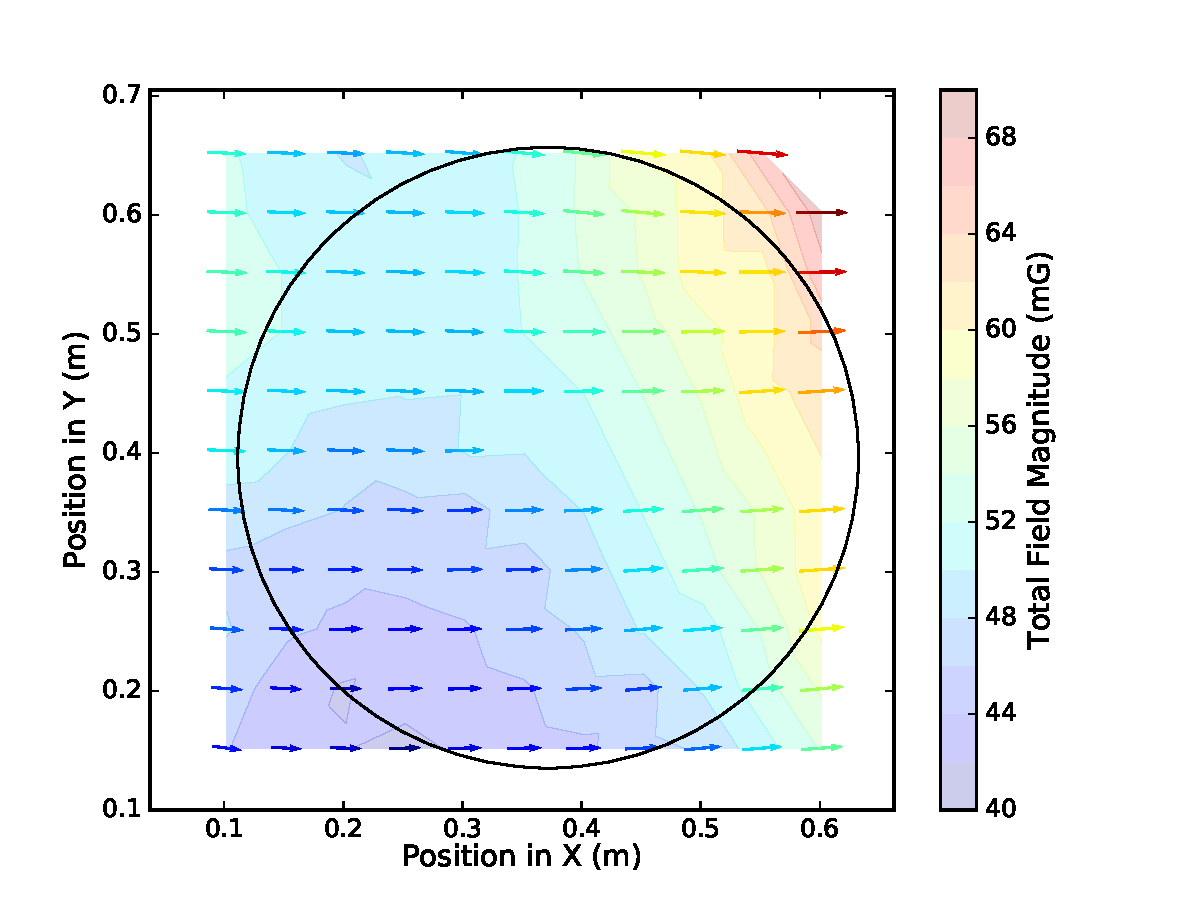
\includegraphics[width=0.5\textwidth]{bfield_rep_Bx50_z700_1_vec.pdf}
    }
    \subfloat[Trial 2: magnetic field magnitude and vector field\label{fig:bfield_rep_Bx50_2_vec}]{
      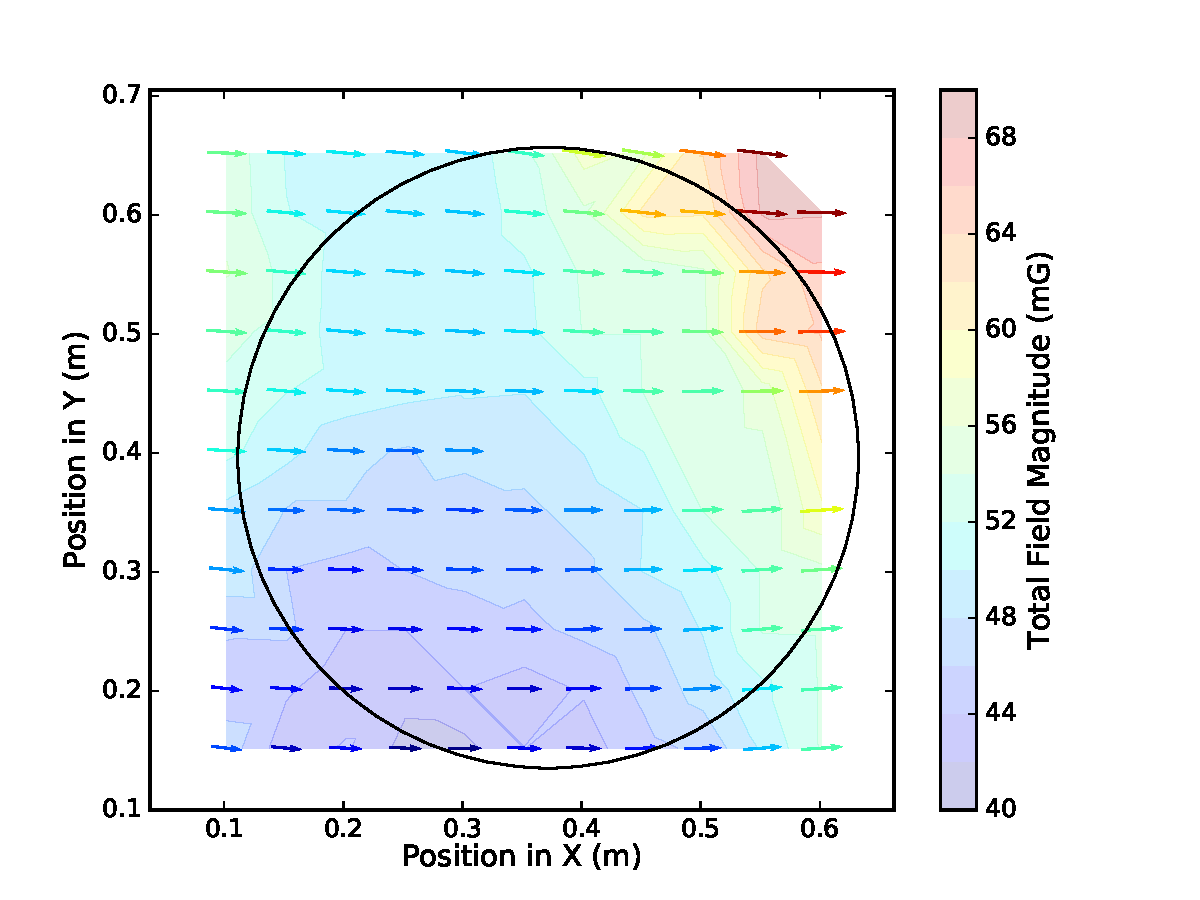
\includegraphics[width=0.5\textwidth]{bfield_rep_Bx50_z700_2_vec.pdf}
    }\\
    \vspace{-3 mm}
    \subfloat[Trial 1: x-component of magnetic field\label{fig:bfield_rep_Bx50_1_x}]{
      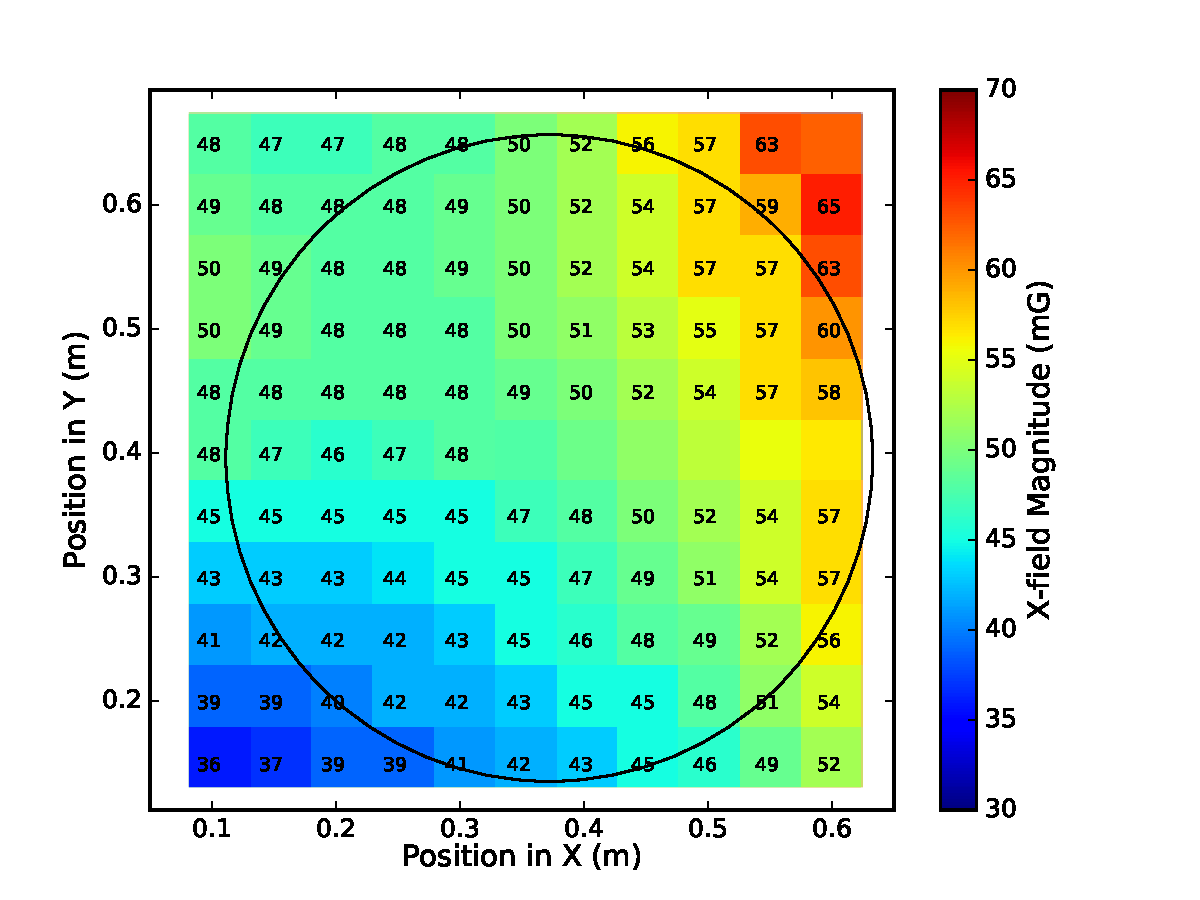
\includegraphics[width=0.5\textwidth]{bfield_rep_Bx50_z700_1_x.pdf}
    }
    \subfloat[Trial 2: x-component of magnetic field\label{fig:bfield_rep_Bx50_2_x}]{
      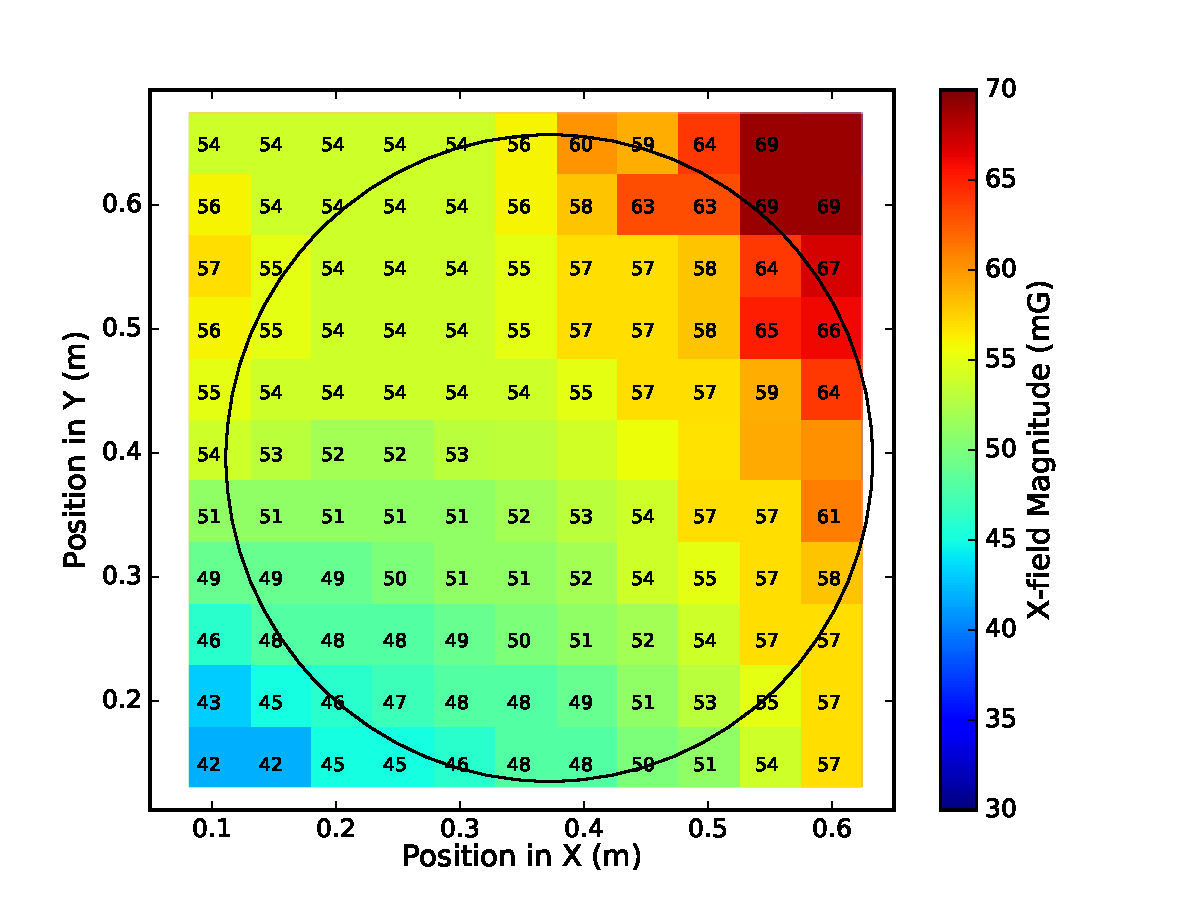
\includegraphics[width=0.5\textwidth]{bfield_rep_Bx50_z700_2_x.pdf}
    }
  \caption{Plots of magnetic field with an offset of 50 mG in the x-direction.}
  \label{fig:bfield_rep_Bx50}
  \end{center}
\end{figure}
%
%
\begin{figure}[hp]
  \begin{center}
    \subfloat[Trial 1: magnetic field magnitude and vector field\label{fig:bfield_rep_By150_1_vec}]{
      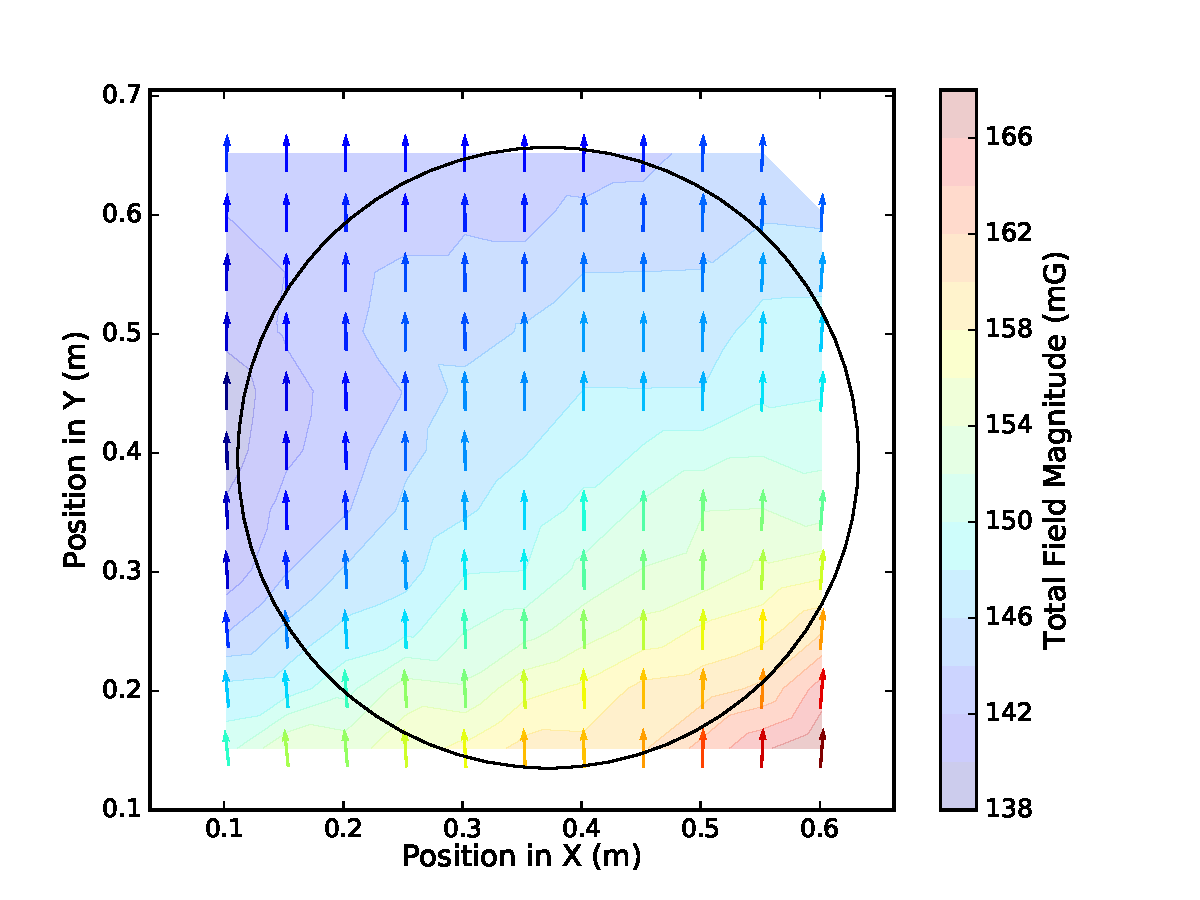
\includegraphics[width=0.5\textwidth]{bfield_rep_By150_z700_1_vec.pdf}
    }
    \subfloat[Trial 2: magnetic field magnitude and vector field\label{fig:bfield_rep_By150_2_vec}]{
      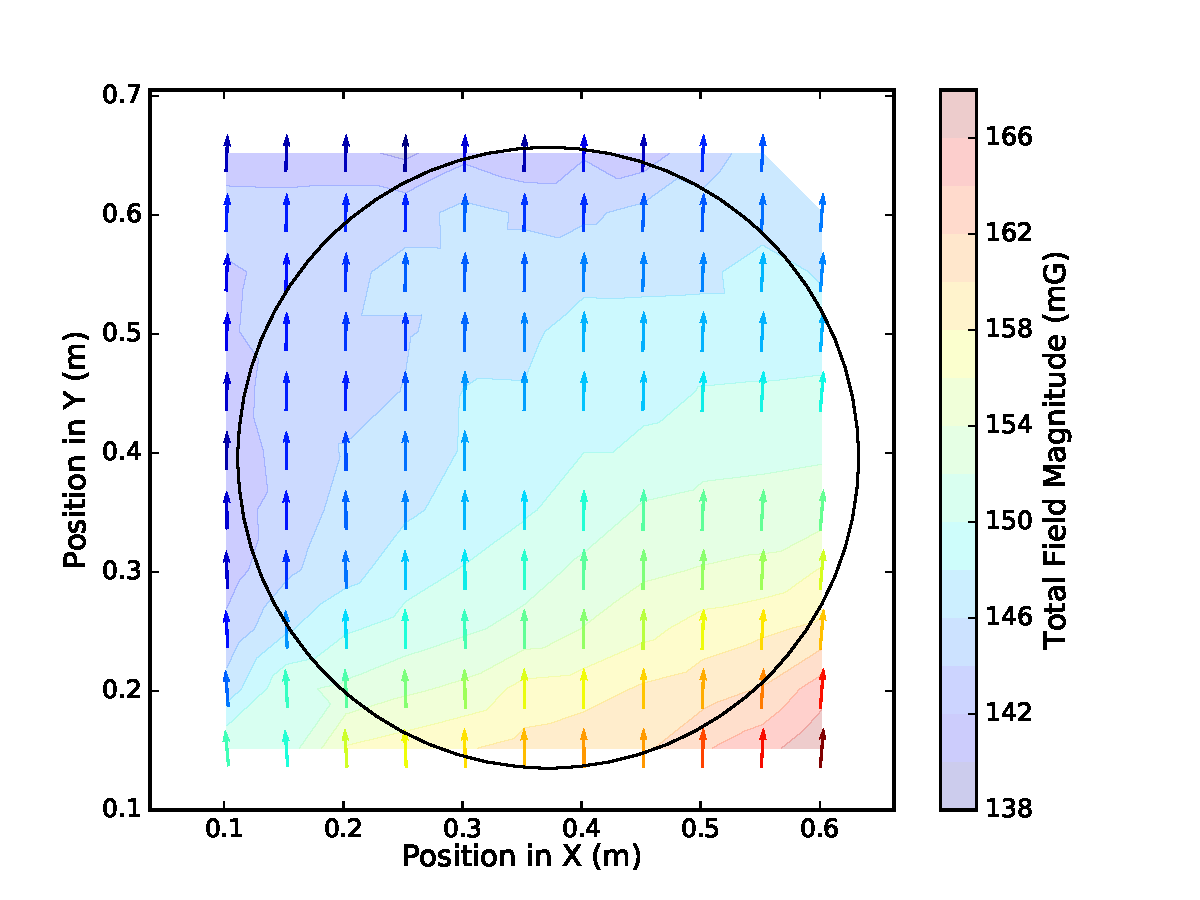
\includegraphics[width=0.5\textwidth]{bfield_rep_By150_z700_2_vec.pdf}
    }\\
    \vspace{-3 mm}
    \subfloat[Trial 1: y-component of magnetic field\label{fig:bfield_rep_By150_1_y}]{
      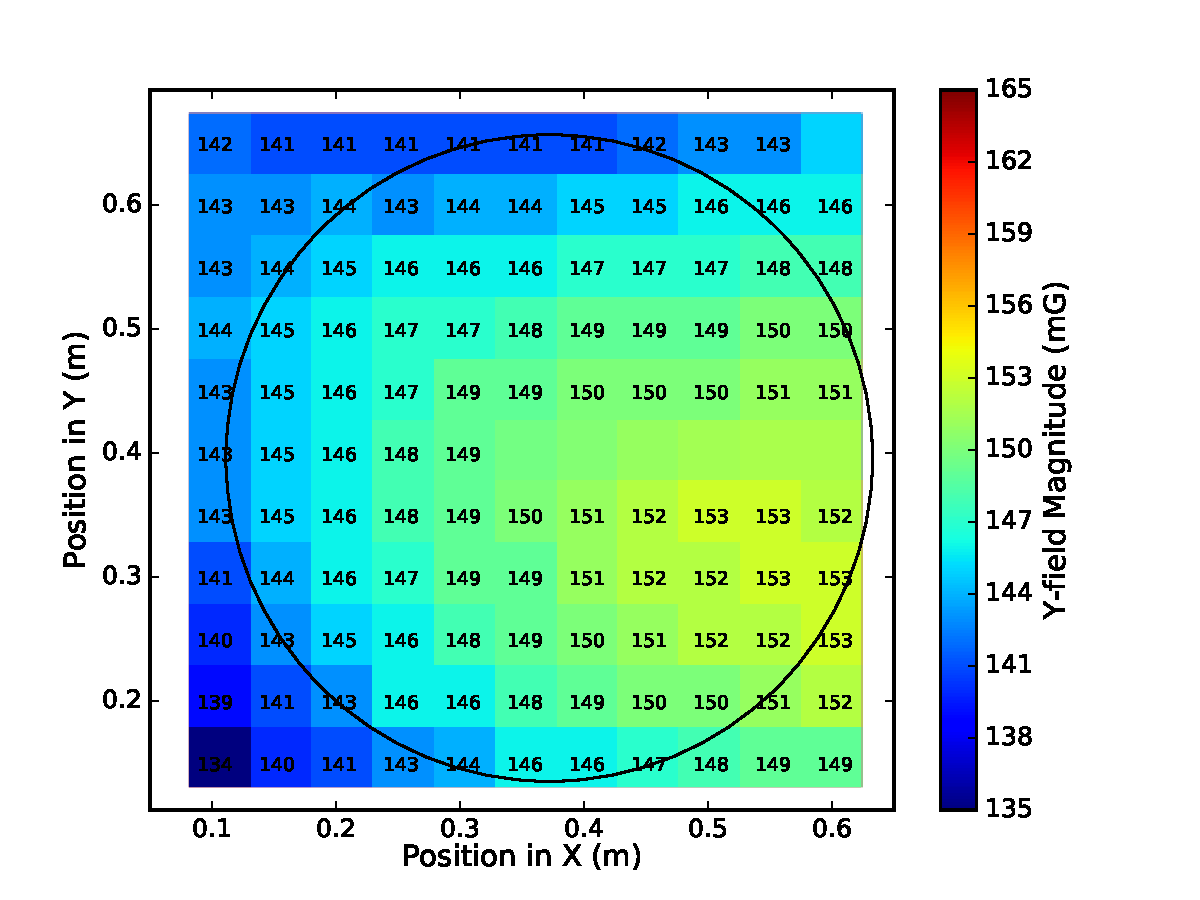
\includegraphics[width=0.5\textwidth]{bfield_rep_By150_z700_1_y.pdf}
    }
    \subfloat[Trial 2: y-component of magnetic field\label{fig:bfield_rep_By150_2_y}]{
      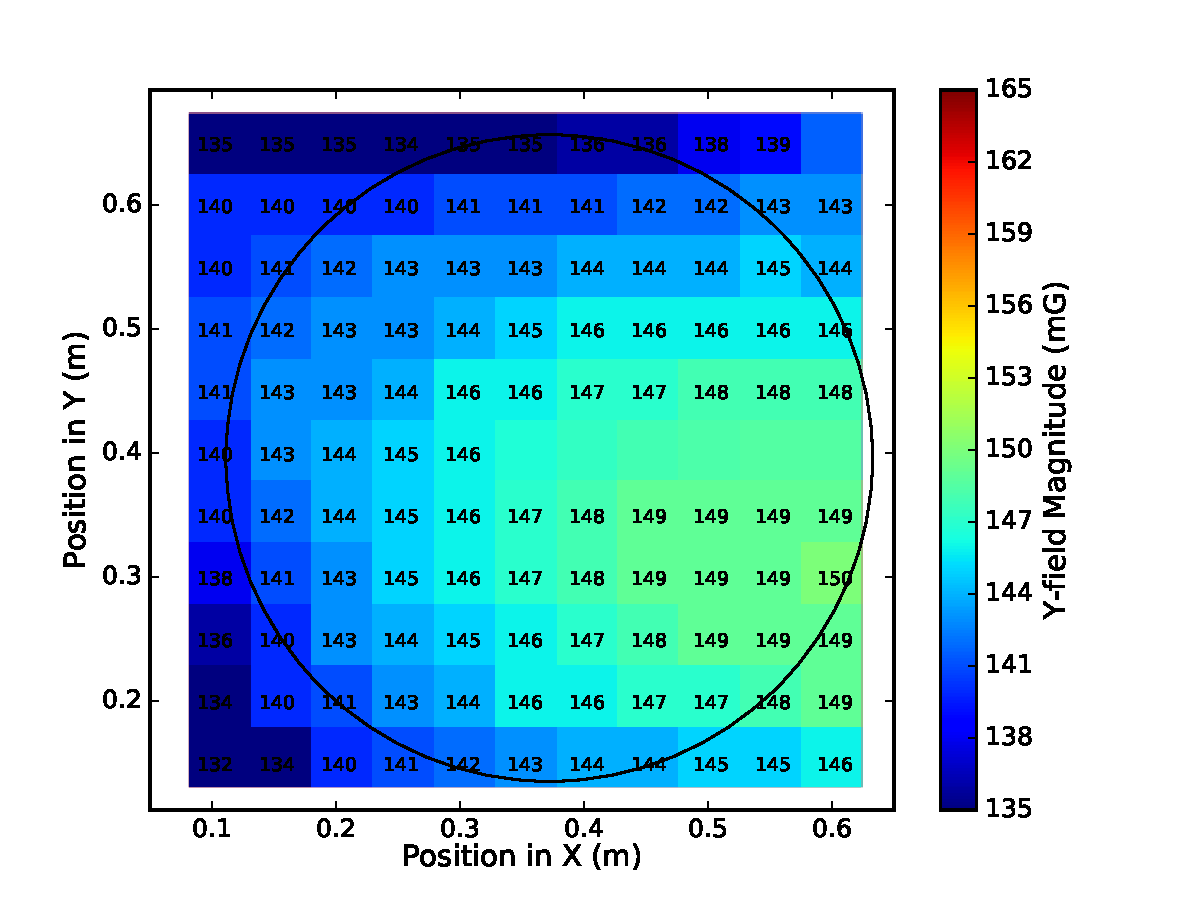
\includegraphics[width=0.5\textwidth]{bfield_rep_By150_z700_2_y.pdf}
    }
  \caption{Plots of magnetic field with an offset of 150 mG in the y-direction.}
  \label{fig:bfield_rep_By150}
  \end{center}
\end{figure}
%
%
\begin{figure}[hp]
  \begin{center}
    \subfloat[Trial 1: magnetic field magnitude and vector field\label{fig:bfield_rep_Bzn100_1_vec}]{
      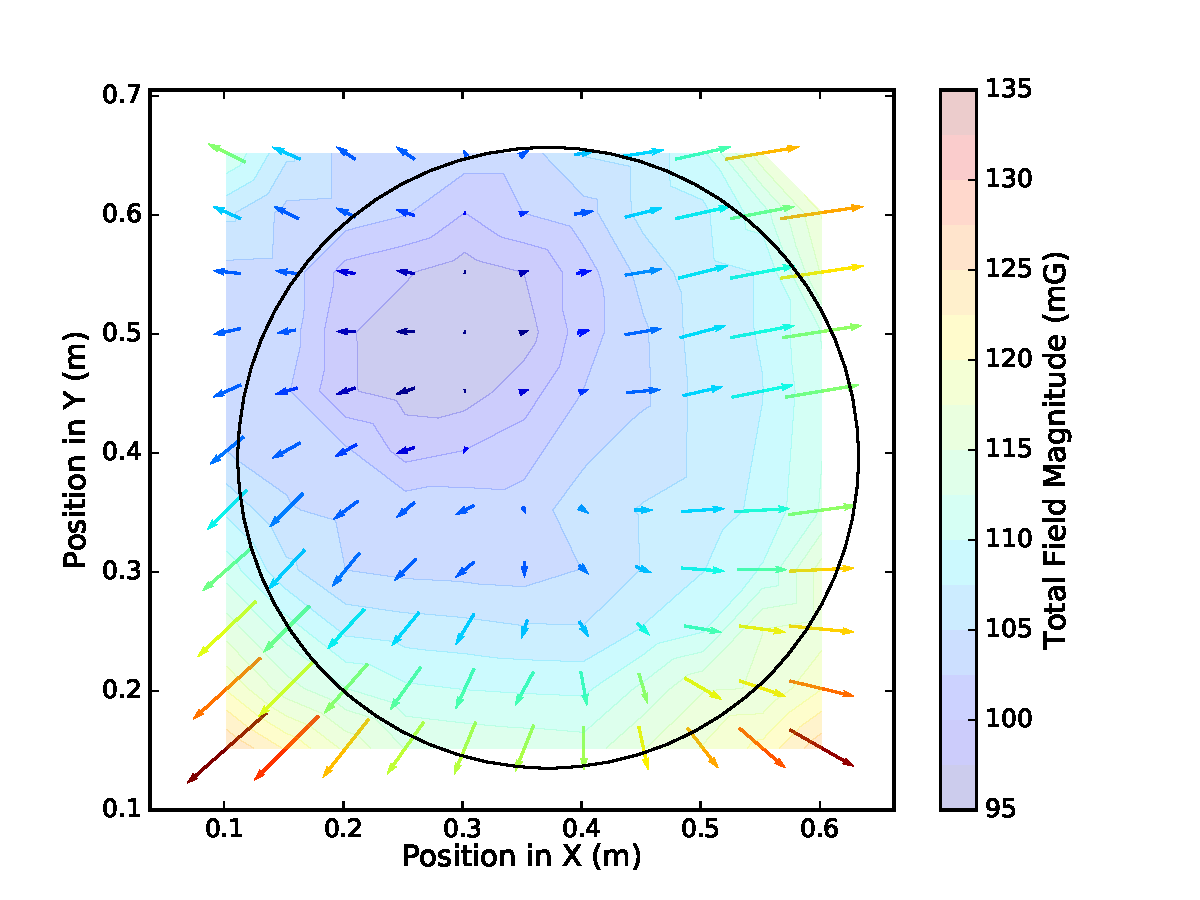
\includegraphics[width=0.5\textwidth]{bfield_rep_Bzn100_z700_1_vec.pdf}
    }
    \subfloat[Trial 2: magnetic field magnitude and vector field\label{fig:bfield_rep_Bzn100_2_vec}]{
      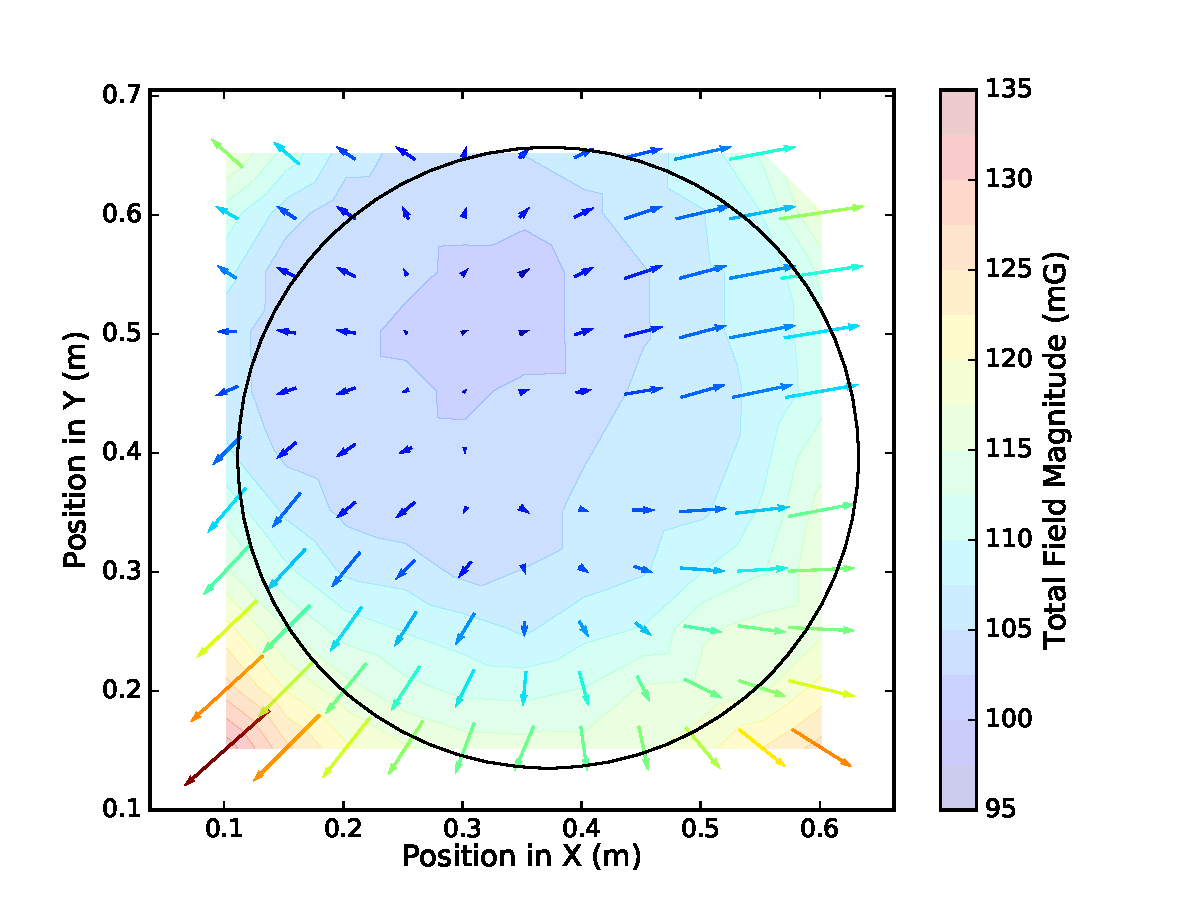
\includegraphics[width=0.5\textwidth]{bfield_rep_Bzn100_z700_2_vec.pdf}
    }\\
    \vspace{-3 mm}
    \subfloat[Trial 1: z-component of magnetic field\label{fig:bfield_rep_Bzn100_1_z}]{
      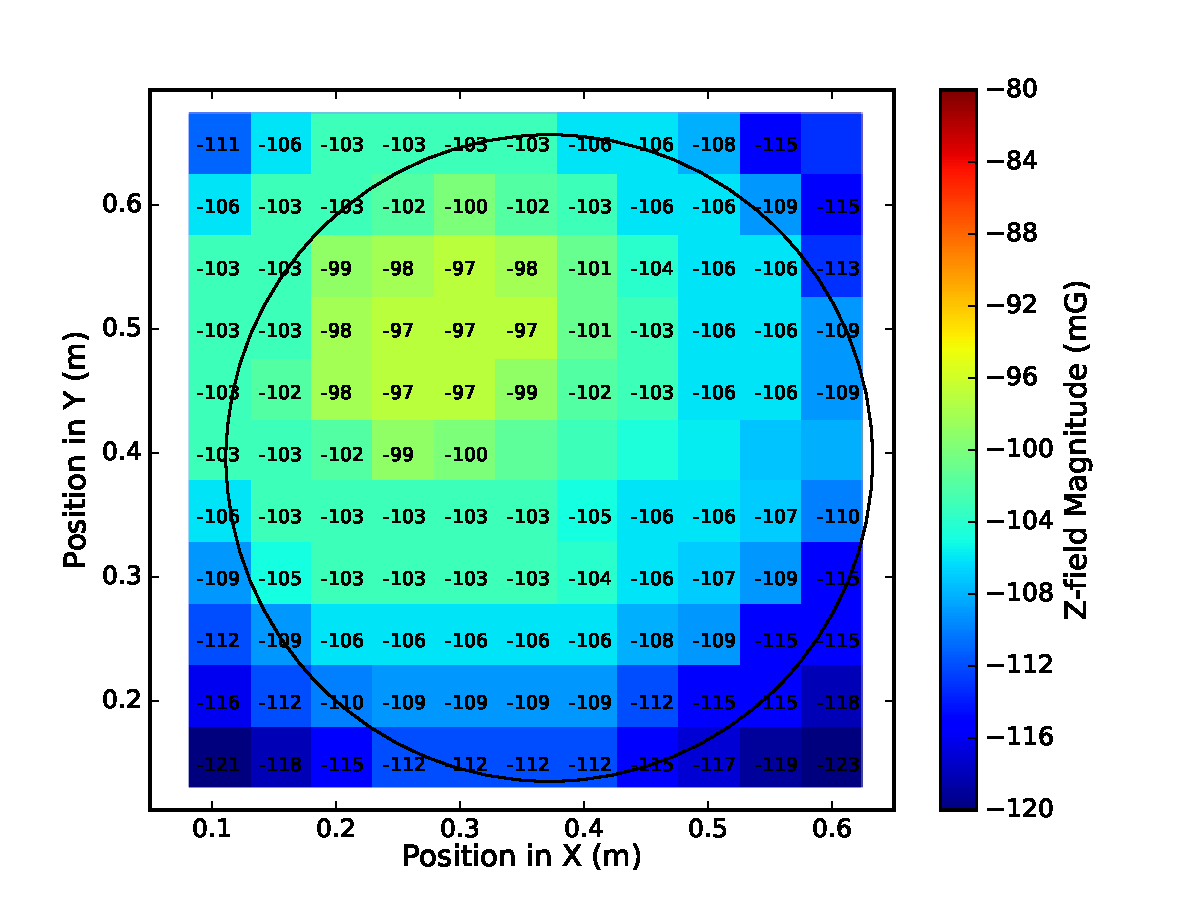
\includegraphics[width=0.5\textwidth]{bfield_rep_Bzn100_z700_1_z.pdf}
    }
    \subfloat[Trial 2: z-component of magnetic field\label{fig:bfield_rep_Bzn100_2_z}]{
      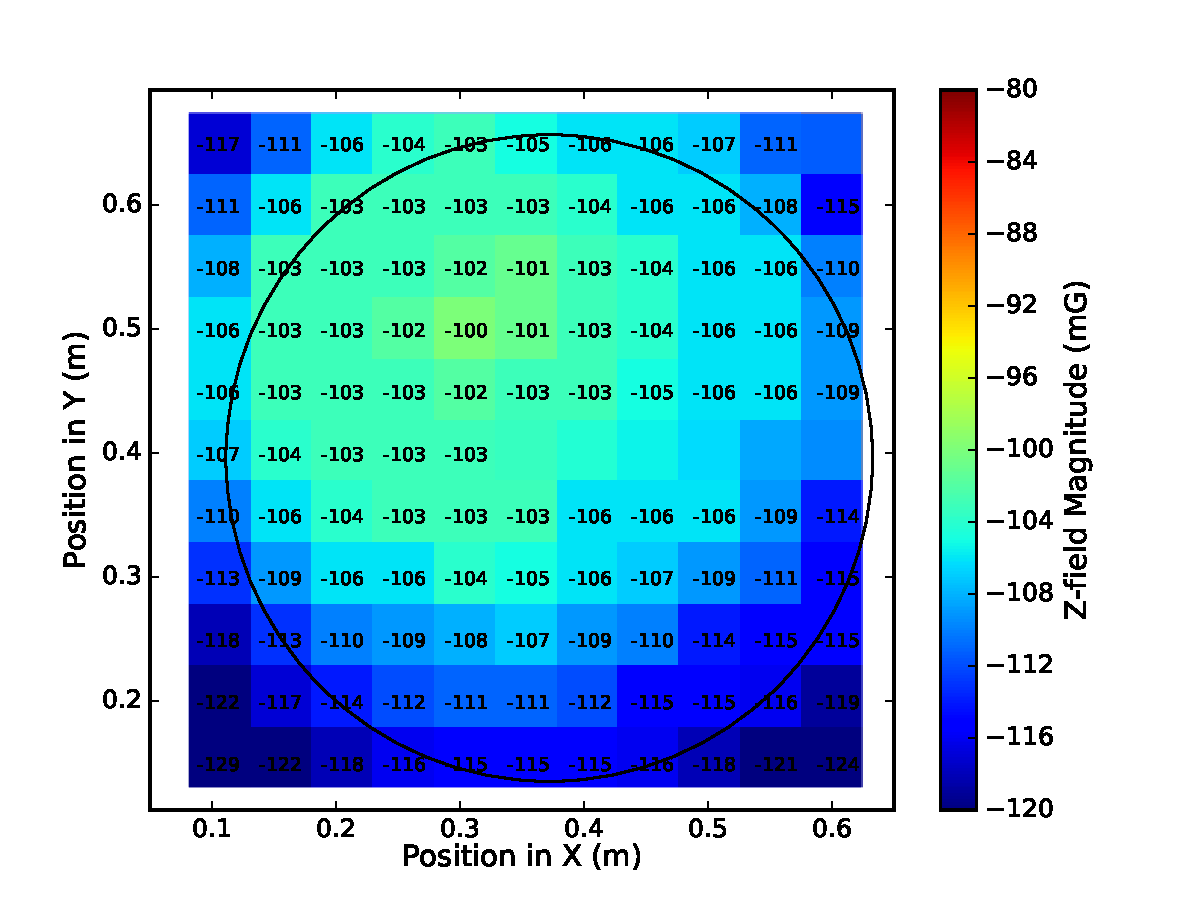
\includegraphics[width=0.5\textwidth]{bfield_rep_Bzn100_z700_2_z.pdf}
    }
  \caption{Plots of magnetic field with an offset of -100 mG in the z-direction.}
  \label{fig:bfield_rep_Bzn100}
  \end{center}
\end{figure}
%
\newpage



%% References
%%
%% Following citation commands can be used in the body text:
%% Usage of \cite is as follows:
%%   \cite{key}         ==>>  [#]
%%   \cite[chap. 2]{key} ==>> [#, chap. 2]
%%

%% References with BibTeX database:

\bibliographystyle{elsarticle-num}
\bibliography{PTF.bib}

\end{document}
